
\documentclass{article} % For LaTeX2e
\usepackage{iclr2027_conference,times}
\usepackage{graphicx}
% Optional math commands from https://github.com/goodfeli/dlbook_notation.
\input{math_commands.tex}
\usepackage{booktabs}
\usepackage{bbm}
\usepackage{multirow}
\usepackage[
    colorlinks=true,
    citecolor=blue,
    linkcolor=blue,
    urlcolor=blue,
    backref=page
]{hyperref}
\usepackage{amssymb}

\renewcommand*{\backref}[1]{}
\renewcommand*{\backrefalt}[4]{%
  \ifcase #1
    No citations.%
  \or
    pg #2.%
  \else
    pgs #2.%
  \fi
}
\usepackage{url}

\usepackage[table]{xcolor}

% ============================================================
% Author comments
% ============================================================
\newif\ifcomments
\commentstrue        % Show all comments
% \commentsfalse     % Hide all comments

% Generic comment command
\newcommand{\authorcomment}[3]{%
  \ifcomments
    \textcolor{#1}{\textbf{#2:} #3}%
  \fi
}

% Authors
\newcommand{\rks}[1]{\authorcomment{brown}{RK}{#1}} %Ravi
\newcommand{\ms}[1]{\authorcomment{red}{MS}{#1}} %Medha
\newcommand{\nr}[1]{\authorcomment{teal}{NR}{#1}} % Nikhita
\newcommand{\vkv}[1]{\authorcomment{orange}{VK}{#1}} % Kesav
\newcommand{\db}[1]{\authorcomment{violet}{DB}{#1}} % Digbalay

%\title{AnimateBanana: Transforming Process Diagrams into Animated Narratives}

\title{
\textsc{AnimateBanana}:%
\hspace{0.25em}%
\raisebox{-0.22\height}{%
  
\includegraphics[height=1.15em]{pipeline_diagrams/animatebanana_logo.png}%
}%
\hspace{0.35em}%
Transforming Process Diagrams into Animated Narratives
}

% Authors must not appear in the submitted version. They should be hidden
% as long as the \iclrfinalcopy macro remains commented out below.
% Non-anonymous submissions will be rejected without review.

\author{Antiquus S.~Hippocampus, Natalia Cerebro \& Amelie P. Amygdale \thanks{ Use footnote for providing further information
about author (webpage, alternative address)---\emph{not} for acknowledging
funding agencies.  Funding acknowledgements go at the end of the paper.} \\
Department of Computer Science\\
Cranberry-Lemon University\\
Pittsburgh, PA 15213, USA \\
\texttt{\{hippo,brain,jen\}@cs.cranberry-lemon.edu} \\
\And
Ji Q. Ren \& Yevgeny LeNet \\
Department of Computational Neuroscience \\
University of the Witwatersrand \\
Joburg, South Africa \\
\texttt{\{robot,net\}@wits.ac.za} \\
\AND
Coauthor \\
Affiliation \\
Address \\
\texttt{email}
}

% The \author macro works with any number of authors. There are two commands
% used to separate the names and addresses of multiple authors: \And and \AND.
%
% Using \And between authors leaves it to \LaTeX{} to determine where to break
% the lines. Using \AND forces a linebreak at that point. So, if \LaTeX{}
% puts 3 of 4 authors names on the first line, and the last on the second
% line, try using \AND instead of \And before the third author name.

\newcommand{\fix}{\marginpar{FIX}}
\newcommand{\new}{\marginpar{NEW}}

\newcommand{\benchCount}{$5000$~}

%\iclrfinalcopy % Uncomment for camera-ready version, but NOT for submission.
\begin{document}


\maketitle

\begin{abstract}
Diagrams are often used to communicate scientific processes visually. However, conveying process dynamics and explanatory flow from a static diagram remains challenging. Although animated narratives improve comprehension and engagement, creating them is a manual and time-consuming process. We present \textbf{\textsc{AnimateBanana}}, a framework for automatically transforming process-oriented scientific diagrams into animated narratives. Given a diagram and a user-specified presentation style, \textsc{AnimateBanana} generates an editable animation-aware programmatic representation enriched with narration cues. Specialized reasoning stages operate on this representation to produce a narration-infused animation plan, which is subsequently synthesized into the final animated narrative. The generated narratives are faithful to the source diagram, controllable, and deployable across multiple presentation formats (PDF, SVG, GIF, MP4, and PPTX). To support this new task, we introduce \textbf{AnimateBench},
a curated benchmark of \benchCount process-oriented diagrams with verified animated narratives spanning diverse diagram families, presentation styles, and levels of structural complexity, including expert-derived reference narratives where available. We further introduce task-specific metrics for
evaluating both the resulting narratives and their intermediate representations. Automated evaluation and controlled user studies show that \textsc{AnimateBanana} consistently outperforms competing baselines in narrative quality, providing empirical support for  animation-aware representations and modular reasoning for narrative generation. 
\end{abstract}

\section{Introduction}


Scientific diagrams are used to communicate neural architectures, scientific workflows, algorithms, and engineering systems. While the underlying concepts are often dynamic, the visual medium itself is static. Consequently, readers must infer information flow, temporal progression, and causal relationships from a static image. Even with accompanying reference text, readers or viewers must mentally reconstruct the underlying process and its dynamics.

To compensate for these shortcomings, researchers, educators, and industry practitioners routinely animate diagrams during presentations. Prior work in multimedia learning has shown that suitably designed animated presentation strategies improve comprehension, knowledge retention, and reduce cognitive load~\citep{mayer2003cognitiveload,rey2019segmenting,xie2017cueingmeta,
schneider2023whiteboard}. However, creating animated narratives remains largely manual. Authors must decide what to present, when to present, how to guide the viewer's attention, and what to explain at each stage. Producing high-quality animated narratives  requires substantial effort and specialized authoring tools.

Recent advances in multimodal foundation models have enabled impressive progress in scientific figure generation, editing, and executable graphics generation. Diagram-to-code systems recover editable programmatic representations from raster images~\citep{starvector,detikzify}, while other systems generate or modify publication-quality scientific illustrations~\citep{paperbanana,figagent,autofigure,livefigure}. However, requirements for animated narratives go beyond  editable graphic generation. Other efforts have explored narrated presentations from documents or structured content~\citep{shi-etal-2025-presentagent,code2video}, where the visual presentation is constructed around the generated narrative. Our setting is more constrained: the animation and narration must remain grounded in the elements, structure, and spatial organization of an existing scientific diagram. Generating an animated narrative therefore requires recovering this structure, identifying coherent presentation units, determining their order and granularity, and coordinating the resulting visual progression with narration text . Together, these requirements define a new task: \emph{diagram-conditioned animated narrative generation}.

To this end, we introduce \textsc{AnimateBanana}, a modular framework of specialized multimodal agents that transforms a static process-oriented scientific diagram into an animated narrative. \textsc{AnimateBanana} first generates an editable, \underline{animation-aware} programmatic representation that exposes the diagram's visual elements and structure for downstream reasoning. Subsequent agents identify coherent presentation units, plan their order and granularity, generate accompanying narration, and synthesize the final animation. Critic-guided feedback progressively verifies and refines these representations throughout the pipeline. 
Explicit symbolic representations of diagram entities, structural relationships, and presentation metadata guide the downstream reasoning process, while the source diagram provides
additional visual grounding where required. When available, \textsc{AnimateBanana} exploits auxiliary context such as figure captions and source document to improve presentation planning. 

Overall, the representations enable faithful and editable animated narratives with explicit control over animation style. Additionally, the narratives can be rendered into multiple deployment formats  (SVG, GIF, MP4, PPTX). This enables the resulting narratives to be reused across papers, presentations, online media, and interactive learning environments without manual re-authoring for each medium. Uniquely, \textsc{AnimateBanana} can produce narratives that render natively inside standard PDF viewers, transforming conventional PDF documents into interactive visual experiences.

To support this emerging task, we introduce \textbf{AnimateBench}, the first benchmark for process-oriented scientific diagram animation and narration. AnimateBench comprises \benchCount curated process-oriented diagrams together with verified animated narratives, including expert-derived reference narrations where available. We further introduce task-specific metrics for
evaluating both final animated narratives and the intermediate representations
used to generate them. We also investigate the utility of auxiliary context such as figure captions and source documents for improving presentation planning and narration on complex diagrams. AnimateBench enables systematic evaluation of both the final animated narrative and the intermediate representations produced during its generation. Experiments demonstrate that \textsc{AnimateBanana} outperforms strong baselines while substantially reducing authoring effort. User studies further show that \textsc{AnimateBanana}'s animated narratives are highly preferred by human evaluators.

We have used \textsc{AnimateBanana} to generate animated narratives for diagrams in this paper. Additional examples and details can be found in supplementary material.


\section{Related Work}

\noindent\textbf{Diagram-to-code and programmatic representations:}
Recent work has explored generation of programmatic representations (e.g.,
SVG, TikZ) from raster images~\citep{starvector,renderingaware,geosvgrl,
belouadi2023automatikz,belouadi2024detikzify}. More recent approaches
incorporate explicit reasoning, iterative rendering, and visual feedback to
improve the structural coherence and fidelity of generated vector
graphics~\citep{wang2026reliable,liang2026render}. These approaches primarily
target visually faithful, structured, and editable reconstruction or
generation. In contrast, \textsc{AnimateBanana} optimizes for animated narrative generation rather than direct diagram reconstruction.


\noindent\textbf{Scientific diagram generation and understanding:}
Recent advances in multimodal foundation models have accelerated research on scientific visual communication, including systems for generating posters, presentation slides, and scientific illustrations from research papers~\citep{posteragent,pptagent,ge2025autopresent,shi-etal-2025-presentagent}. More recently, several agentic systems have explored generation, editing, and refinement of publication-quality editable scientific figures~\citep{paperbanana,figagent,autofigure,scifig,livefigure,vfig}. Recent work has also studied scientific image synthesis through programmatic generation, using explicit understanding and planning stages to improve structural and scientific correctness~\citep{lin2026scientific}. Complementary efforts have explored explicit intermediate representations for diagram understanding~\citep{explicitdiagram}, representation learning for computer science diagrams~\citep{rlcsdia}, diagram parsing through structural alignment~\citep{alignmentdiagram}, hierarchical layout recovery~\citep{layoutrecovery}, and benchmark datasets for scientific
diagrams~\citep{diagrambank}. However, these works fundamentally treat scientific diagrams as static visual artifacts. They do not address the problem of inferring presentation structure and transforming process-oriented diagrams into animated narratives.



\noindent\textbf{Animated narratives and agentic generation:}
A complementary line of work studies animated visual narratives in data visualization and motion graphics~\citep{dataplayer,dataplaywright,narrativeplayer,zheng2025designspace}. Approaches include motion generation from single images~\citep{mggen}, narrated data videos~\citep{dataplayer,
dataplaywright,narrativeplayer}, and narration-centric authoring~\citep{wonderflow}. Some recent systems generate editable animations over structured vector graphics~\citep{keyframer,logomotion}, with VAnim~\citep{liang2026vanim} further introducing structure-preserving vector
animation. Other systems generate narrated presentations or educational videos~\citep{shi-etal-2025-presentagent,code2video}. These settings either focus on animating graphical assets or afford greater freedom in constructing the visual presentation. In contrast, \textsc{AnimateBanana} must determine
what to present, in what order, and what to narrate while remaining grounded in an existing scientific diagram. Recent agentic visual-generation systems such as GenAgent~\citep{jiang2026genagent} and SceneOrchestra~\citep{he2026sceneorchestra} use multimodal reasoning, tool orchestration, and iterative refinement, but for static image and scene generation. More broadly, agentic frameworks such as ReAct, AutoGen, and MetaGPT provide general abstractions for
reasoning and task decomposition~\citep{yao2023react,wu2024autogen,hong2024metagpt}. \textsc{AnimateBanana} instead uses a structured plan--execute--critique workflow with representations and transformations specialized for diagram-conditioned animated narrative generation.

\begin{figure}
    \centering
    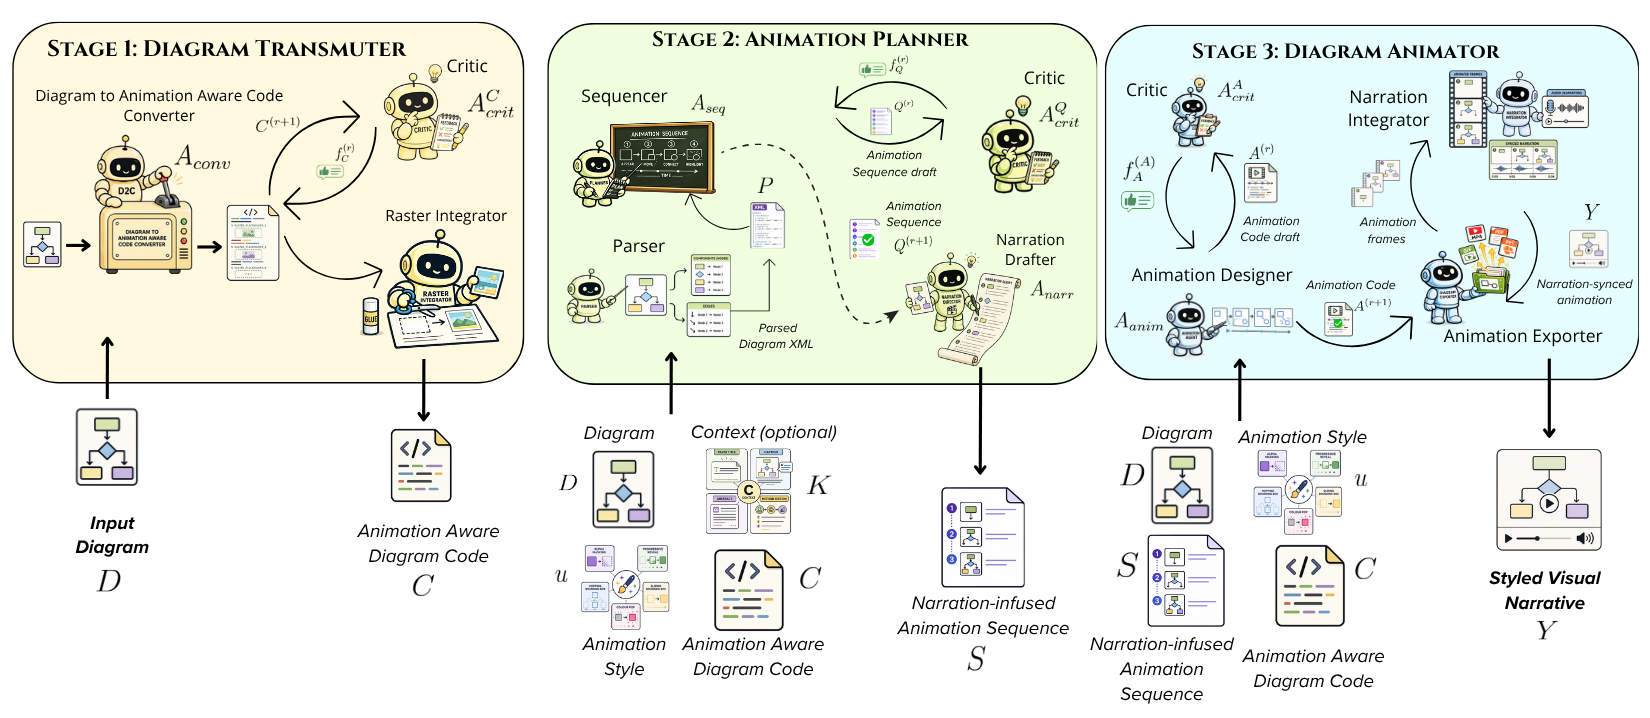
\includegraphics[width=\linewidth]{pipeline_diagrams/High Level Overview Diagram_not.png}
    % \vspace{-0.35cm}
    \caption{A High-Level Overview of the
     \textsc{AnimateBanana} pipeline}
    \vspace{-0.35cm}
    \label{fig:pipeline}
\end{figure}

\section{\textsc{AnimateBanana}}

Given a static process-oriented diagram $D$, a user-specified animation style $u$, and optional auxiliary context $K$, our goal is to generate an animated narrative $Y$:
\[
Y=\mathcal{F}(D,u;K),
\]
By default, $K=\varnothing$. When available, $K$ may include the figure caption or relevant source document text. The animation
style $u$ specifies how the visual progression is realized. Choices include
\emph{Progressive Reveal}, which incrementally reveals elements from a blank
canvas; \emph{Hopping Box} and \emph{Sliding Box}, which discretely or
continuously move a focus box across successive elements; \emph{Color Pop},
which progressively restores color to elements of an initially grayed-out
diagram; and \emph{Alpha Masking}, which progressively unmasks elements of an initially masked diagram. Each style may optionally be augmented with
pan--zoom effect over the region currently being presented.

Rather than generating the narrative directly, \textsc{AnimateBanana} uses a multi-stage agentic framework that progressively constructs representations tailored to animation and narration. As illustrated in Figure~\ref{fig:pipeline}, the framework comprises three stages. The \textit{Diagram Transmuter} converts $D$ into animation-aware diagram code $C$, where visual elements are addressable and organized for downstream animation. The \textit{Animation Planner} reasons over $C$ to obtain a narration-infused animation sequence $S$ that specifies presentation order, grouping, granularity, and accompanying narration, optionally informed by $K$. The \textit{Diagram Animator} utilizes $S$ along with code $C$ and style $u$ to synthesize the final animated narrative $Y$. Throughout the process, specialized multimodal agents construct and iteratively refine these representations through critic-guided feedback. 

\subsection{Stage-I: Diagram Transmuter}

As shown in Figure~\ref{fig:pipeline}, the \textit{Diagram Transmuter} converts the input diagram $D$ into animation-aware diagram code $C$. Unlike conventional diagram-to-code conversion, the objective is not direct reconstruction alone. The generated code incorporates persistent markers and animation-related metadata that support subsequent presentation planning, narration, and animation.

To achieve this, the Converter agent $\mathcal{A}_{\mathrm{conv}}$ generates an initial representation $C^{(0)}=\mathcal{A}_{\mathrm{conv}}(D)$, assigning persistent semantic identifiers to animatable elements such as nodes, edges, text labels, and composite elements. For example, a processing block and its connecting arrows remain separately addressable even when they form part of a larger module. The identifiers also encode structural roles and allow animation attributes, such as visibility, appearance time, and duration, to be associated with individual elements. Thus,  code $C$ preserves the visual organization of diagram $D$ while providing explicit handles for subsequent presentation planning and animation.


Since $C$ is used throughout the subsequent stages, errors in its visual or structural content can propagate to animation planning. At refinement round $r$, the Critic agent $\mathcal{A}_{\mathrm{crit}}^{C}$ evaluates the rendered $C^{(r)}$ against $D$ and produces feedback $f_C^{(r)}=\mathcal{A}_{\mathrm{crit}}^{C}(D,C^{(r)})$ on semantic content, containment, layout, style, and relative proportions. The Converter then revises the representation as $C^{(r+1)}=\mathcal{A}_{\mathrm{conv}}(D,C^{(r)},f_C^{(r)})$. As shown by the Converter--Critic loop in Figure~\ref{fig:pipeline}, refinement continues until the rendering satisfies a fidelity threshold or a maximum number of rounds is reached.

Scientific diagrams can also contain photographs, icons, plots, and other visually complex regions that are poorly suited to programmatic reconstruction. The Raster Integrator preserves such regions directly from diagram $D$. During code generation, these regions are represented by identifiable placeholders. The corresponding regions are then extracted from $D$ and inserted into $C$ while preserving their position and identity. This allows diagram code $C$ to combine programmatically represented elements with raster content without requiring the latter to be reconstructed.


\subsection{Stage II: Animation Planner}

As shown in Figure~\ref{fig:pipeline}, the \textit{Animation Planner} transforms animation-aware diagram code $C$ generated by Stage I into a narration-infused animation sequence $S$. Although $C$ makes diagram elements individually addressable, it does not specify how they should be presented. A coherent animation requires decisions about which elements should appear together, their presentation order and granularity, and how the visual progression should be explained. The Animation Planner makes these decisions independently of the  animation style.

The first processing step in the Animation Planner is the Parser (Figure~\ref{fig:pipeline}), which converts animation-aware diagram code $C$ into a structured XML representation $P$. While $C$ retains the information required for faithful rendering and animation, $P$ abstracts away rendering-specific details while preserving diagram entities, their connections, and hierarchical relationships. Hierarchy is particularly relevant to presentation granularity, since a module may be introduced as a whole or through its constituent elements at different points in the narrative. Overall, the resulting XML provides a compact representation over which presentation decisions can be made.

Given the parsed XML representation $P$, the Sequencer agent $\mathcal{A}_{\mathrm{seq}}$ constructs an initial presentation sequence $Q^{(0)}=(q_1,\ldots,q_T)$, where each $q_t$ contains one or more elements to be introduced at step $t$. The Sequencer must choose among alternative groupings and traversal orders while accounting for structural dependencies and hierarchy. For example, connected elements may be introduced together, while a composite module may be presented before its internal components. At refinement round $r$, the Sequence Critic $\mathcal{A}_{\mathrm{crit}}^{Q}$ evaluates $Q^{(r)}$ for coverage and presentation coherence and produces feedback $f_Q^{(r)}=\mathcal{A}_{\mathrm{crit}}^{Q}(P,Q^{(r)})$. The Sequencer revises its proposal as $Q^{(r+1)}=\mathcal{A}_{\mathrm{seq}}(P,Q^{(r)},f_Q^{(r)})$ until the sequence is validated or the refinement limit is reached. As part of this process, style $u$ is used to select the correct subset of elements (e.g. blocks, arrows, text labels) to be introduced for each member $q_t$ of the validated sequence.

Finally, the Narration Drafter agent $\mathcal{A}_{\mathrm{narr}}$ generates narration text $n_t$ for each presentation step $q_t$, yielding $S=((q_1,n_1),\ldots,(q_T,n_T))$. The agent determines what should be explained at each step from the newly introduced elements and the preceding presentation history, keeping the narration synchronized with the evolving visual state. The resulting narration-infused animation sequence $S$ couples what is presented with what is explained. When available, auxiliary context $K$, such as the figure caption or source document, provides additional semantic information for this decision, particularly when an element's role is not evident from the diagram alone.

\subsection{Stage III: Diagram Animator}

As shown in Figure~\ref{fig:pipeline}, the \textit{Diagram Animator} utilizes the narration-infused animation sequence $S$ to obtain the final animated narrative $Y$.  %The same animation plan can also be instantiated over either TikZ or SVG using representation-specific rendering mechanisms, with TikZ supporting animated PDF output and SVG supporting browser-native animation.
Given $S$, the animation-aware code $C$, and a user-specified style $u$, the Animation Designer agent $\mathcal{A}_{\mathrm{anim}}$ generates an initial executable animation program $A^{(0)}=\mathcal{A}_{\mathrm{anim}}(C,S,u)$. The agent determines how each presentation step should be realized under $u$ while preserving the sequence and visual organization specified by the preceding stages.

The generated program is rendered into frames and evaluated by the Animation Critic $\mathcal{A}_{\mathrm{crit}}^{A}$ against the source diagram. At refinement round $r$, the Critic produces feedback $f_A^{(r)}=\mathcal{A}_{\mathrm{crit}}^{A}(D,S,A^{(r)},M^{(r)})$ on visual and temporal errors, including incorrect visibility, unintended motion, occlusion, and deviations from the planned presentation order. The critic memory $M^{(r)}$, shown in Figure~\ref{fig:pipeline}, records feedback and attempted corrections from previous rounds. The Animation Designer uses both the current feedback and this history to select a revised solution, producing $A^{(r+1)}=\mathcal{A}_{\mathrm{anim}}(C,S,u,A^{(r)},f_A^{(r)},M^{(r)})$. Refinement continues until the animation is validated or the maximum number of rounds is reached.

Once validated, $A$ is rendered into the visual states required by the target presentation style. The Animation Exporter converts these states into the requested deployment format, including PDF, SVG, GIF, MP4, or PPTX.  In parallel, the Narration Integrator associates the step-level narration in $S$ with the corresponding visual states, using speech synthesis where audio narration is required. The final narrative $Y$ therefore retains the presentation and narration decisions encoded in $S$ while adapting their realization to the target style and output format. 

\noindent \textit{Implementation Note:} In our implementation, the diagram code (C) is represented as SVG. The representation follows an animation-aware contract that assigns persistent identifiers to diagram entities and encodes their semantic roles, hierarchy, relationships, and raster regions. This metadata is subsequently parsed into the XML representation used by the Animation Planner, while the original SVG geometry is retained for animation and rendering. Representation-specific implementation details are provided in the supplementary material.



\section{AnimateBench: Benchmarking Scientific Diagram Animation}
\label{sec:animatebench}

% FigureBench 
% Paper2Fig
% PaperBanana
% Sci-Fig
% Sci-MMIR
% We scraped from Papers2Code
% FlowLearn

We introduce \textbf{AnimateBench}, a benchmark of 5,000 process-oriented scientific diagrams spanning four animation styles, yielding 20,000 animated narratives. For this, we first curate process-oriented diagrams from scientific papers spanning computer vision, machine learning, information retrieval, bioinformatics, computer networking and related areas. We focus on figures that communicate pipelines, architectures, workflows, and other structured processes. The selection is guided by diversity in structural and visual characteristics, including element density, connectivity, hierarchical depth, layout organization, and the presence of raster content. We also collect the corresponding conference presentation videos when available. We temporally localize the portion in which the figure is explained and spatially crop the video to the diagram region, retaining the accompanying transcript. The resulting presentation sequence serves as a nominal reference for validating the narrative in the benchmark counterpart.

Constructing rich animation annotations at this scale entirely manually is prohibitively expensive. We therefore use \textsc{AnimateBanana} to bootstrap the annotation process, with human intervention and correction at intermediate stages of the pipeline. For each diagram, we generate narratives in all four animation styles and randomly select one for detailed human verification. Annotators inspect its presentation sequence, narration, and animation, revising intermediate artifacts when necessary to ensure correct content coverage and adherence to the specified animation style.

Beyond the final animation, AnimateBench retains the presentation sequence, step-level narration, and animation style. We also retain the available source context for each diagram, including its figure caption and relevant paper content. Finally, we retain intermediate representations produced during construction, including the hierarchy-aware XML, animation-aware diagram code, and executable animation code. This provides multiple levels of annotation for analyzing both the resulting narrative and the intermediate decisions leading to it.

Figure~\ref{fig:animatebench_overview} summarizes the scale and composition of AnimateBench. It highlights diversity along both diagram dimensions and narrative dimensions. The figure also summarizes the retained annotations and the use of conference presentations as external references where available. 

\begin{figure}
    \centering
    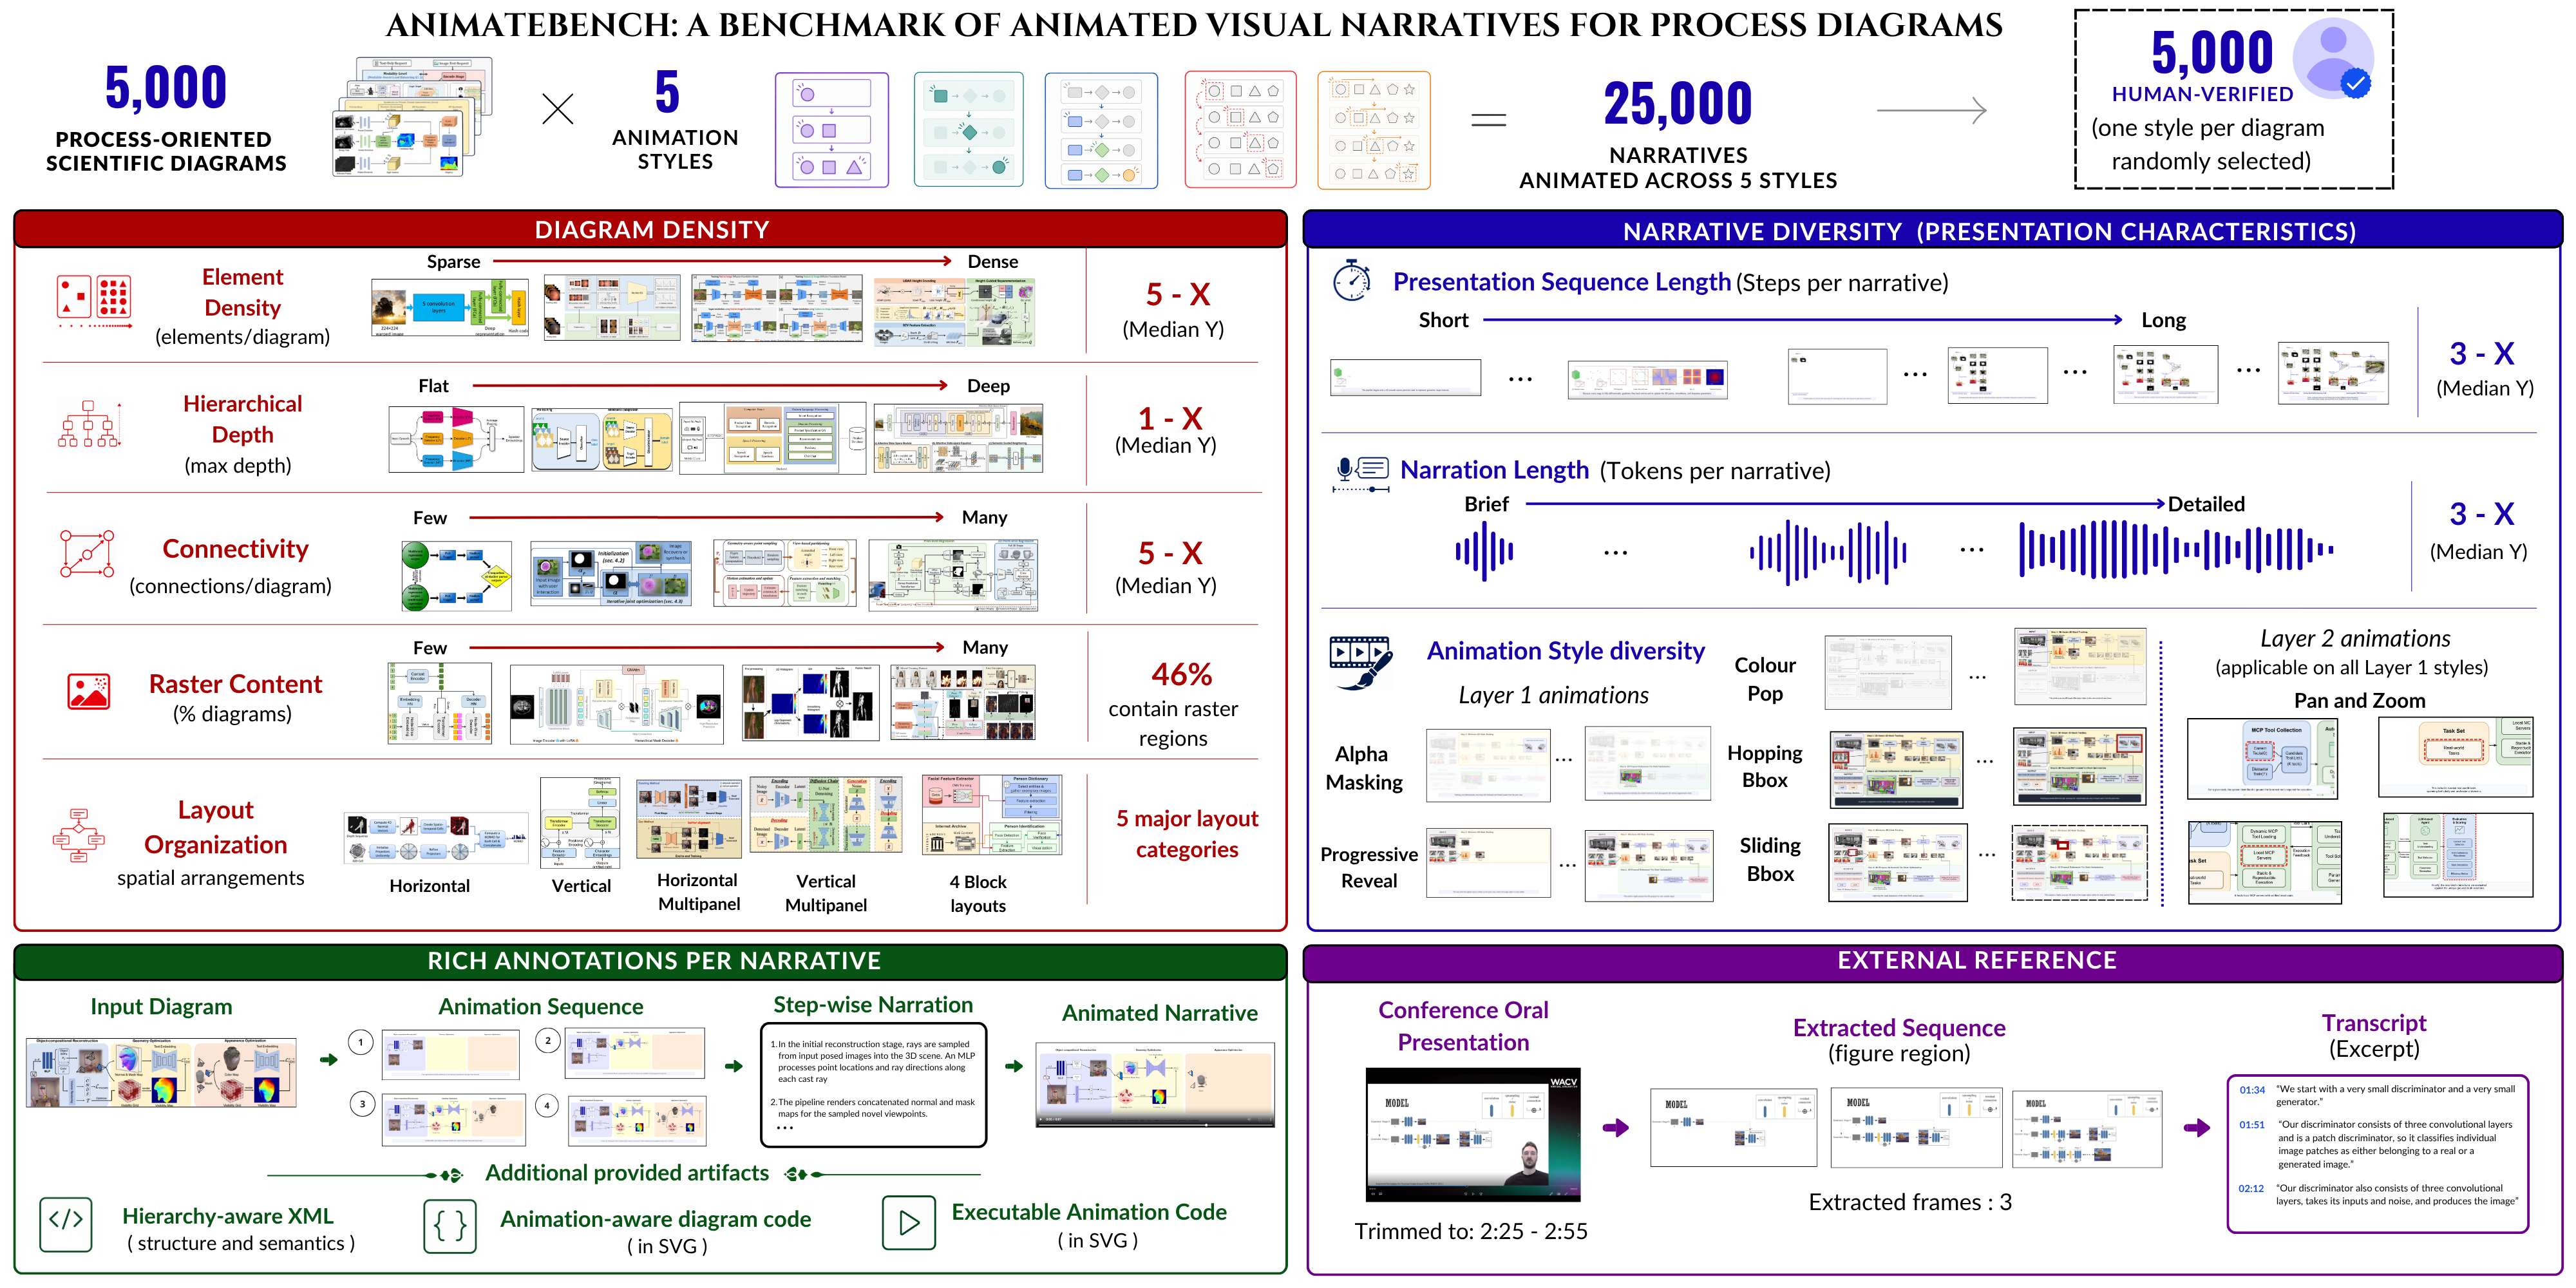
\includegraphics[width=\linewidth]{pipeline_diagrams/AnimateBench Diagram.png}
    % \vspace{-0.35cm}
    \caption{A High-Level Overview of the
     AnimateBench}
    \vspace{-0.35cm}
    \label{fig:animatebench_overview}
\end{figure}


% \begin{table}[t]
%     \centering
%     \caption{\textbf{AnimateBench statistics.} 
%     The benchmark spans substantial variation in diagram complexity and
%     animated narrative structure.}
%     \label{tab:animatebench_statistics}
%     \small
%     \setlength{\tabcolsep}{4pt}
%     \begin{tabular}{llcc}
%         \toprule
%         \textbf{Category} & \textbf{Statistic} & \textbf{Median} & \textbf{Range} \\
%         \midrule

%         \multirow{4}{*}{Diagram}
%             & Elements                         & XX & XX--XX \\
%             & Connections                      & XX & XX--XX \\
%             & Hierarchy depth                  & XX & XX--XX \\
%             & Raster content (\%)              & \multicolumn{2}{c}{XX.X\%} \\
%         \midrule

%         \multirow{3}{*}{Narrative}
%             & Presentation steps               & XX & XX--XX \\
%             & Elements / step                  & XX & XX--XX \\
%             & Narration length (words)         & XX & XX--XX \\
%         \midrule

%         \multicolumn{2}{l}{Scientific diagrams} &
%             \multicolumn{2}{c}{5,000} \\
%         \multicolumn{2}{l}{Animation styles} &
%             \multicolumn{2}{c}{4} \\
%         \multicolumn{2}{l}{Animated narratives} &
%             \multicolumn{2}{c}{20,000} \\
%         \multicolumn{2}{l}{Human-verified narratives} &
%             \multicolumn{2}{c}{5,000} \\
%         \multicolumn{2}{l}{Conference presentation references} &
%             \multicolumn{2}{c}{XXX} \\
%         \bottomrule
%     \end{tabular}
% \end{table}

% \section{Evaluation Metrics}
% \label{sec:metrics}

% %Existing metrics do not capture the structural and temporal decisions involved in scientific diagram-conditioned animated narrative generation. 
% We introduce task-specific metrics that evaluate systems at multiple levels, separating the quality of final animated narrative from the intermediate decisions and representations used to produce it. Specifically, we evaluate
% (i) the \emph{final animated narrative} for visual fidelity, content coverage,
% and animation-style compliance; (ii) the \emph{animation sequence} for the
% quality and structural consistency of presentation decisions; (iii) the
% \emph{structured representation} for the correctness of diagram entities,
% hierarchy, and relationships; and (iv) the \emph{programmatic representation}
% for executability and rendering fidelity. Intermediate metrics are reported
% only for systems that expose the corresponding artifacts. Detailed rubrics and judge implementations are provided in the supplementary material.

% % We evaluate diagram-to-animation systems at four levels: the final animated
% % narrative, the presentation sequence, the structured XML representation, and the executable programmatic code. Final-output metrics apply to all systems, while intermediate and code-level metrics apply when the corresponding pipeline artifacts are available. Detailed rubrics and judge implementations are provided in the supplementary material.

% \subsection{Final Animated Narrative}
% Evaluating the final animation employs a two-stage funnel: strict elimination gates followed by a granular sequence assessment. Given a source diagram $D$, requested style $u$, and animation $Y$, \texttt{Visual Fidelity} measures the preservation of the source layout, geometry, proportions, and text integrity, while \texttt{Style Compliance} verifies adherence to the rules of $u$. The \texttt{Omitted Elements Criterion} (OEC) ensures $Y$ completely covers the necessary diagram entities in $D$. For animations that survive these initial checks, the \texttt{Selection Sensibility Score} (SSS) evaluates whether the elements highlighted at each timestep form a logically coherent presentation unit. The \texttt{Granularity and Pacing Score} (GPS) measures whether the volume and intrinsic complexity of the introduced information remain digestible. Both metrics aggregate 0--4 timestep-level judgments, normalized to $[0,100]$. Their equally weighted average forms the \texttt{Base Animation Quality Score (BAQS)}. The final \texttt{Animation Quality Score} (AQS) is then derived by applying a bounded flat penalty to the BAQS for any unjustified repetition of elements.

% \subsection{Animation Sequence}
% For an animation sequence $S=(S_1,\ldots,S_T)$, \texttt{Element Coverage} measures both recall and precision over the elements animated by the reference sequence, capturing omitted and extraneous elements, respectively. \texttt{Traversal-Order Fidelity (TOF)} measures whether the realized sequence order adheres to a pre-decided traversal strategy, without imposing a single preferred ordering. \texttt{Dependence-Order Violation Rate (DOVR)}
% measures the fraction of edges introduced before their source element and, \texttt{Style-Schema Compliance} verifies the inclusion and exclusion constraints imposed by the selected animation style $u$.

% \subsection{Structured and Programmatic Representations}
% For the structured XML representation of $D$, \texttt{Parent Assignment Accuracy} measures whether sub-container elements are assigned to their correct hierarchical parents. \texttt{Edge Topology F1} evaluates the relational accuracy of connected elements, while \texttt{Depth Violations} captures structurally inconsistent nesting depths.\\
% For diagram codes in SVG, \texttt{Rendering Fidelity} evaluates how faithfully the output reproduces $D$, weighting logical layout and containment most heavily. Concurrently, the \texttt{Diagram Component Score} measures the accuracy of the semantic classes assigned to elements within the code itself.\\
% Finally, for programmatic animation code, \texttt{Animation Integration Footprint (AIF)} measures the code-level invasiveness of an animation by evaluating the extent to which the existing diagram code must be modified to accomodate the animation logic.



% % \section{Evaluation metrics}

% % % \textsc{AnimateBench} evaluates diagram-to-animation systems by tracing the generation process in reverse. Rather than just evaluating the final video, we assess the pipeline backwards: from the final animated narrative to the presentation sequence, and finally down to the underlying structured diagram representation. This artifact-level approach isolates a system's performance across three key dimensions: visual fidelity, presentation planning, and the executability of the generated code (both for diagram reconstruction and animation rendering).

% % % Using this backward-tracing methodology, 

% % We introduce a novel suite of metrics tailored to each stage of narrative generation.

% % \subsection{Final Animation Evaluation}
% % Evaluating the final animation requires a two-stage "funnel" approach. First, animations must pass a strict set of elimination gates designed to catch fundamental generation failures. Only animations that pass these checks are evaluated for the quality of their presentation sequence. The surviving animations are scored for the nuance of their sequencing and pacing with a bounded penalty for unnecessary repetition.

% % \subsubsection{Elimination-based Metrics}
% % The elimination stage checks three basic requirements: fidelity to the source
% % diagram, compliance with the specified animation style, and coverage of the
% % diagram elements that should appear in the animation. Failing any of these removes the animation from further evaluation:
% % \paragraph{Visual Fidelity Score (VFS)}
% % Measures how accurately the animation preserves the source diagram's geometry, style, proportions, and text integrity. We use a VLM as a judge at both the frame and video levels to ensure consistency, eliminating animations that fall below a baseline threshold.
% % \paragraph{Animation Style Compliance Score (ASCS)}
% % Verifies that the animation faithfully obeys the rules of its target style. We evaluate each frame against a strict style-behavior checklist; any deviation triggers elimination.
% % \paragraph{Omitted Elements Criterion(OEC)}
% % Ensures complete diagram content coverage. By comparing the generated sequence against an exhaustive ground-truth checklist, we eliminate any animation that drops necessary diagram entities or connections.
% % \subsubsection{Animation sequence quality}
% % For animations that clear the elimination gates, we evaluate the underlying presentation logic using the diagram's ground-truth XML schema, rather than relying solely on rendered visual heuristics. We calculate a Base Animation Quality Score (BAQS) derived from two equally weighted metrics, and then apply a penalty for unneccessary repetition.
% % \paragraph{Selection Sensibility Score (SSS)}
% % Assesses whether the elements highlighted at each timestep make logical sense. SSS evaluates \emph{element appropriateness} (respecting hierarchy and structural dependencies) and \emph{group coherence} (grouping elements that form a meaningful semantic or logical unit). Each timestep is scored on a 0–4 scale, ranging from Severe Violation to Fully Sensible.
% % \paragraph{Granularity and Pacing Score (GPS)}
% % Measures whether the volume of animated elements introduced at each timestep forms a digestible presentation unit. It considers both the \emph{volume} of newly targeted elements and their \emph{intrinsic complexity}. Rather than penalizing sparse presentations, GPS weights intrinsic structural complexity more heavily than raw element counts. Each timestep receives a 0–4 score, ranging from Severe Overload to Well-Paced.\\


% % The timestep-level SSS and GPS bands are averaged across the animation and normalized to a 0–100 scale. These two normalized scores contribute equally to the Base Animation Quality Score (BAQS).

% % \paragraph{Unnecessary repetition penalty}
% % We additionally penalize unnecessary repetitions of already animated elements. Persistence across frames is not considered repetition, nor are legitimate revisits such as returning to a central hub or revisiting a parent while presenting its child nodes. Only unjustified repetitions contribute to the penalty.

% % Let $R$ denote the number of unjustified repetitions. The final Animation
% % Quality Score (AQS) is

% % \[
% % \mathrm{AQS}
% % =
% % \mathrm{BAQS}
% % -
% % \min(pR,P_{\max}),
% % \]

% % where $p$ is the penalty per unnecessary repetition and $P_{\max}$ bounds the
% % total penalty.
% % \subsection{Intermediate Representation Evaluation}
% % The intermediate representations produced by the animation planner are evaluated at two levels: the \emph{animation sequence}, which specifies how the diagram is traversed and presented, and the \emph{structured XML representation}, which specifies the elements and relationships over which this traversal is defined.
% % We propose metrics to evaluate the animation sequence first, followed by the XML schema. 
% % \subsubsection{Animation Sequence Evaluation}
% % A well-planned sequence must not only target the correct elements but also reveal them in a structurally coherent order that respects the chosen animation style.
% % \paragraph{Element Coverage (Precision \& Recall)}
% % We measure coverage across two axes in a style-aware manner. Recall ensures the generated sequence touches all necessary elements present in the reference presentation, penalizing dropped content. Precision identifies hallucinated or extraneous elements not found in the ground truth.

% % \paragraph{Traversal-Order Fidelity (TOF).}
% % Validating \textit{what} is shown is insufficient; we must also validate \textit{when} it is shown. TOF measures how strictly the sequence adheres to its declared traversal strategy. Rather than imposing a single universal order, it verifies intent, for example, ensuring an "overview-first" style prioritizes top-level elements, while a "detail-first" style completes a specific structural unit before moving on.

% % % I feel the following metric should be omitted, it is perfectly fine to show an edge before its target element is displayed, we can modify the metric such that we count for cases where the edge is displayed before its source element is displayed. Or if everyone agrees we can just get rid of this metric.
% % \paragraph{Dependence-Order Violation Rate (DOVR).}
% % Visual narratives must respect structural dependencies. We define a dependency violation specifically as an edge being introduced before its source element. While drawing an edge before its target is often a valid stylistic choice to build anticipation, an edge preceding its origin breaks logical causality and creates a relation without a visual referent.
% % \paragraph{Style-Schema Compliance.}
% % A binary pass/fail check verifying that the sequence obeys the hard inclusion and exclusion rules of its selected animation style

% % \subsubsection{XML Schema Evaluation}
% % The animation sequence operates over the XML schema of the
% % diagram. Consequently, the sequence quality is inextricably linked to the accuracy of the underlying XML. We evaluate this structural backbone across three dimensions:
% % \paragraph{Parent-Assignment Accuracy.}
% % For elements successfully aligned between the prediction and the ground truth, this measures the fraction assigned to the correct hierarchical parent, assessing whether the XML preserves the diagram's hierarchical organization. 
% % \paragraph{Edge Topology F1.}
% % Evaluates the relational accuracy of the diagram, specifically verifying whether predicted arrows connect the correct source and target elements.
% % \paragraph{Depth Violations.}
% % Identifies malformed nesting by measuring the fraction of elements whose declared depth is inconsistent with their hierarchy (i.e., penalizing any child whose depth is not exactly one increment greater than its parent's).
% % \subsection{Code-Level Evaluation}
% % We finally evaluate the executable code generated during both the \emph{Diagram Transmutation} stage and at the \emph{Animation Design} stage. We evaluate for both SVG and TikZ, with compilation serving as an immediate validity gate for TikZ.
% % \subsubsection{Diagram Code Evaluation}
% % \paragraph{Diagram Compilation Success Rate (For TikZ)}
% % A binary pass/fail metric measuring whether the generated diagram code successfully compiles. This serves as the absolute prerequisite for the remaining visual evaluations.

% % \paragraph{Rendering Fidelity.}
% % For compilable code, this evaluates how accurately the rendered output reproduces the source figure. While it assesses semantic content, style, and element proportion, it heavily weights logical layout and containment, as these are paramount for source structure preservation.
% % Unlike basic compiler checks, this metric captures visual defects that are syntactically valid but structurally incorrect

% % \paragraph{Diagram Component Score.}
% % Measures whether the semantic classes assigned to elements in the generated diagram code are correct. A judge evaluates the assigned class of every code-level element as, e.g., a block, node, text, raster, or edge, and the score is the fraction of correctly classified elements.

% % \subsubsection{Animation Code Evaluation}
% % \paragraph{Animation Compilation Success Rate.}
% % The equivalent executability gate for the animation stage, verifying that the injected sequence code successfully compiles and renders the final animation.

% % \paragraph{Animation Integration Footprint.}
% % Measures the structural invasiveness of adding animation to the static diagram. AIF is calculated as the ratio of pre-existing diagram lines modified or deleted to the total number of animation-specific lines added. Lower AIF values indicate an elegant, purely additive integration, meaning the animation is cleanly layered over the diagram rather than destructively rewriting its underlying representation. This provides a quantifiable way to compare how naturally different rendering paradigms (such as SVG versus TikZ) accommodate animations.

% % \section{Experiments}
% % To comprehensively evaluate \textsc{AnimateBanana}, we conduct (i) automated evaluations using our proposed \textsc{AnimateBench} protocol, (ii) a human evaluation study assessing visual quality and practical utility, and (iii) controlled ablations isolating the contributions of key pipeline modules. Detailed qualitative case studies and implementation details are provided in the Appendix.
% % \subsection{Automated Evaluations}
% % \label{subsec:automated_evaluations}
% % We benchmark \textsc{AnimateBanana} against a diverse spectrum of baseline models, including open-source models, proprietary models, and API-accessible models, under two evaluation settings.
% % \begin{itemize}
% %     \item \textbf{Pipeline-Integrated:} Models are slotted into our \textsc{AnimateBanana} pipeline to handle the sub-tasks, exposing the structured intermediate artifacts required for deep evaluation.
% %     \item \textbf{Zero-Shot (End-to-End):} Models are prompted to generate the final animation directly from the source diagram, bypassing explicit intermediate planning or supervision from our pipeline agents.
% % \end{itemize}

% % \paragraph{The \textsc{AnimateBench} Evaluation Suites.}
% % Because evaluation granularity depends entirely on the artifacts a system exposes, we organize our metrics into three complementary suites that correspond to progressively deeper levels of the generation process:
% % \begin{itemize}
% %     \item \textbf{Final Animation Suite (FAS):} Evaluates the ultimate rendered visual narrative. Because every system produces a video, FAS serves as our universal evaluation suite. Zero-shot generators are evaluated \emph{exclusively} under this suite.
% %     \item \textbf{Intermediate Representation Suite (IRS):} Evaluates whether a system correctly parses the diagram's structure and proposes a logical animation sequence for its traversal.
% %     \item \textbf{Code-Centric Suite (CCS):} Evaluates the executability and validity of generated diagram and animation code (e.g., TikZ or SVG).
% % \end{itemize}

% % Consequently, pipeline-integrated systems receive a comprehensive diagnosis across all three suites (FAS, IRS, and CCS). In contrast, zero-shot systems are evaluated strictly on their final output (FAS).
% % %reserved for experiment's section
% % %Each baseline's evaluation is performed against the corresponding benchmark artifact, allowing the generated output to be compared at the same level of abstraction as its reference.



% % % \section{AnimateBench: Benchmarking Scientific Diagram Animation}
% % % \label{sec:animatebench}

% % % Scientific diagram animation is a multi-stage task in which the quality of the final animation depends on a sequence of interdependent decisions: faithfully recovering the structure and semantics of the source diagram, deriving a coherent logical order in which its components should be presented, and realizing this plan as a visually and pedagogically effective animation. Consequently, evaluating only the final rendered video provides an incomplete assessment of system performance. A method may produce a seemingly plausible animation while misrepresenting the underlying diagram structure, omitting or redundantly presenting components, or following an incoherent presentation plan. Conversely, programmatic animation systems expose intermediate representations and executable artifacts that provide additional evidence about how the animation is constructed and where errors arise. Existing scientific diagram benchmarks primarily evaluate diagram understanding, text-to-diagram generation, or reconstruction, and do not capture the requirements of the diagram-to-animation task or provide the annotations necessary to evaluate its intermediate stages.\\

% % % To address this evaluation gap, we introduce AnimateBench, a novel benchmark designed for evaluating systems that transform process diagrams into animated narratives. AnimateBench treats diagram-to-animation as a structured generation problem and evaluates systems at multiple levels of the generation process, from intermediate representations and presentation plans to final rendered animations and, when available, executable animation code. Rather than prescribing a specific representation language or implementation paradigm, AnimateBench is organized around the artifacts produced by a system. The evaluation granularity therefore adapts to the artifacts exposed by each method, enabling fair comparison between fundamentally different approaches while allowing systems that provide richer intermediate representations to be evaluated more deeply.
% % % \section{Benchmark Scope}
% % % \label{subsec:animatebench_scope}
% % % AnimateBench is designed to accommodate both emerging end-to-end animation video-generation approaches and structured diagram-to-animation pipelines without privileging a particular implementation paradigm. We distinguish these methods according to the artifacts they might generate during the task. An End-to-end method will directly generate the final animation video without an explicit animation sequence whereas programmatic pipelines (like our \textsc{AnimateBanana}) generate outputs using code-driven languages such as TikZ or SVG, with several structured intermediates along the pipeline. Our benchmark also accounts for the future possibilities of other code-driven languages for the task of diagram to animation and supports the evaluation of their intermediate representations in a structured, code-agnostic manner. This accomodation of both programmatic and non-programmatic approaches to the diagram to animation task is done by the proposal of the following 3 evaluation suites:
% % % \begin{enumerate}
% % %     \item The \textbf{Intermediate Representation Suite (IRS)} evaluates the neccessary intermediate representations that must be generated by a programmatic method in order to convert a diagram into an animation. We focus on the two significant intermediates: a hierarchy-aware structural schema of the diagram and the animation sequence.
% % %     \item The \textbf{Final Animation Suite (FAS)} evaluates the final animation video both on a frame-level and a sequence-level and therefore is applicable to both programmatic pipelines and end-to-end systems.
% % %     \item The \textbf{Code-Centric Suite (CCS)} is specifically designed for programmatic systems that use TikZ or SVG as the representative substrate in their animation pipeline. The measures are reported separately for SVG and TikZ and therefore allows our bench to study the tradeoffs between the different programmatic representations for the task.
% % % \end{enumerate}
% % % Together these evaluation suites provide a comprehensive and layered assessment of diagram-to-animation systems. \textbf{IRS} measures whether a programmatic method displays an understanding of what the diagram contains, how its components are related and uses that insight to plan for an intelligent and meaningful traversal of the diagram. \textbf{FAS} measures the final animation output for its visual coherence, source fidelity and pedagogical value, independent of the underlying generation method and \textbf{CCS} measures whether a programmatic system can reliably realize the intended animation in executable code. Importantly, these suites are complementary rather than competing measures: a system is not required to expose an intermediate representation to participate in final-animation evaluation, while systems that do expose such artifacts receive a more fine-grained diagnosis of their capabilities. This artifact-centric design allows \textsc{AnimateBench} to remain architecture-agnostic at the final-output level while supporting increasingly detailed evaluation as additional system artifacts become available.
% % % \section{Benchmark Curation}
% % % We construct AnimateBench from process-oriented diagrams collected from publicly available research sources, with an emphasis on computer vision, machine learning, and artificial intelligence. Our primary sources include diagrams from papers available on arXiv and papers presented at major research venues such as CVPR, WACV, NeurIPS, and related conferences. We focus specifically on diagrams that communicate a process, pipeline, architecture, workflow, or other structured progression.\\
% % % Rather than stratifying the benchmark solely by scientific domain, we primarily stratify the diagrams according to their structural and visual complexity. Complexity is assessed qualitatively along several complementary dimensions: the density and number of diagram nodes, the complexity of edge connectivity, the degree of nesting and hierarchical depth, the presence and diversity of raster elements such as icons, logos, and other embedded graphics, and the overall layout organization. We additionally account for substantial variation in layout, including different spatial orientations, grouping structures, flow directions, and arrangements of components. Importantly, these dimensions are not treated as independent categories; instead, we deliberately include samples exhibiting different combinations of structural, semantic, and visual complexity to reflect the diversity encountered in real scientific communication.\\
% % % A further consideration in benchmark construction is presentation evidence. In particular, we seek examples for which the original presenter progressively introduces, connects, or elaborates different components of the diagram during the explanation using different animation styles. We  trim the video to the interval in which the diagram is introduced and explained to extract the relevant portion of the presentation and spatially crop it to isolate the relevant visual content. We additionally retain the corresponding presentation transcript. These presentations provide a natural reference for studying how a static scientific diagram can be transformed into an explanatory animated narrative.
% % % \section{Benchmark Composition}
% % % The final benchmark comprises 5,000 manually curated diagram samples. Importantly, the diagrams included in AnimateBench are strictly held out from the data used to develop \textsc{AnimateBanana}. For every benchmark sample, AnimateBench provides a collection of aligned artifacts spanning the different stages of diagram-to-animation. These include:
% % % \begin{enumerate}
% % %     \item Raster Integrated Diagram Code in both SVG and TikZ
% % %     \item Hierarchy-aware XML schema of the diagram
% % %     \item Narration-infused animation sequence
% % %     \item Executable Animation code in both SVG and TikZ
% % %     \item Rendered animation frames
% % %     \item Expert presentation evidence: We provide the temporally and spatially cropped presentation video corresponding to the incremental explanation of the figure, together with its transcript.
% % % \end{enumerate}
% % % To reflect the relative prevalence of animation strategies in scientific presentations, we distribute the 5,000 benchmark samples across five animation styles using a deliberately long-tailed allocation. Progressive reveal constitutes the largest subset (40\%), followed by hopping bounding box (25\%) and sliding bounding box (17.5\%), while colour pop (10\%) and alpha masking (7.5\%) account for smaller but substantial subsets. This distribution prioritizes commonly used presentation mechanisms while retaining sufficient coverage of less frequent styles for style-specific evaluation.
% % % \begin{table}[h!]
% % % \centering
% % % \caption{Visual complexity stratification of \textsc{AnimateBench}. 
% % % Each dimension independently partitions the 5,000 diagrams; therefore, strata across different dimensions are not mutually exclusive. 
% % % For node density, $t$ denotes an empirically determined threshold. (THESE ARE NOT ACTUAL NUMBERS, SIR)\\}
% % % \label{tab:animatebench_complexity}
% % % \small
% % % \begin{tabular}{llrr}
% % % \toprule
% % % \textbf{Complexity Dimension} & \textbf{Stratum} & \textbf{\%} & \textbf{Samples} \\
% % % \midrule

% % % \multirow{2}{*}{Node Density}
% % % & Low ($\leq t$)  & 60.0\% & 3,000 \\
% % % & High ($>t$)     & 40.0\% & 2,000 \\

% % % \midrule

% % % \multirow{2}{*}{Edge Complexity}
% % % & Simple          & 65.0\% & 3,250 \\
% % % & Complex         & 35.0\% & 1,750 \\

% % % \midrule

% % % \multirow{2}{*}{Nesting Depth}
% % % & Shallow ($\leq 2$) & 70.0\% & 3,500 \\
% % % & Deep ($>2$)        & 30.0\% & 1,500 \\

% % % \midrule

% % % \multirow{2}{*}{Raster Content}
% % % & Absent           & 55.0\% & 2,750 \\
% % % & Present          & 45.0\% & 2,250 \\

% % % \midrule

% % % \multirow{5}{*}{Layout Organization}
% % % & Vertical Flow 
% % %   (Top--down / Bottom--up) & 25.0\% & 1,250 \\
% % % & Horizontal Flow 
% % %   (Left--right / Right--left) & 25.0\% & 1,250 \\
% % % & Horizontal Multi-panel & 20.0\% & 1,000 \\
% % % & Vertical Multi-panel   & 15.0\% & 750 \\
% % % & Circular / Cyclic       & 15.0\% & 750 \\

% % % \bottomrule
% % % \end{tabular}
% % % \end{table}
% % % \begin{table}[h!]
% % % \centering
% % % \caption{Distribution of presentation styles in \textsc{AnimateBench}. (THESE ARE NOT ACTUAL NUMBERS, SIR)}
% % % \label{tab:animatebench_styles}
% % % \small
% % % \begin{tabular}{lrr}
% % % \toprule
% % % \textbf{Presentation Style} & \textbf{Percentage} & \textbf{Samples} \\
% % % \midrule
% % % Progressive Reveal       & 40.0\% & 2,000 \\
% % % Hopping Bounding Box     & 25.0\% & 1,250 \\
% % % Sliding Bounding Box     & 17.5\% & 875 \\
% % % Colour Pop               & 10.0\% & 500 \\
% % % Alpha Masking             & 7.5\% & 375 \\
% % % \midrule
% % % \textbf{Total}            & \textbf{100.0\%} & \textbf{5,000} \\
% % % \bottomrule
% % % \end{tabular}
% % % \end{table}
% % % \section{Evaluaton Suite and Metrics}
% % % %Existing scientific diagram benchmarks primarily evaluate understanding, generation, or reconstruction of static figures, and do not provide the annotations needed to evaluate animated narratives. We therefore introduce \textbf{AnimateBench}, a benchmark of \benchCount process-oriented scientific diagrams with verified animated narratives and intermediate annotations for evaluating both presentation planning and final animation quality.

% % % %AnimateBench contains manually curated diagrams excluded from the data used to develop \textsc{AnimateBanana}, and is organized into three complementary subsets. The \emph{Programmatic} subset contains diagrams for which the underlying graphical structure and animation annotations are directly available, enabling controlled evaluation of intermediate and final outputs. The \emph{Real Annotated} subset consists of scientific figures collected from research papers and manually annotated with the structural and presentation information required for evaluation. The \emph{User Study} subset contains selected diagrams together with expert-derived animated narratives and narrations for controlled human evaluation.

% % % %The three subsets support evaluation at different levels of the pipeline, from animation-aware representation and presentation sequencing to the quality of the resulting animated narrative. Figure~\ref{fig:animatebench_overview} summarizes the benchmark construction and annotation process, and Table~\ref{tab:animatebench_statistics} reports the composition of each subset.

% % % \subsection{Tables and Figures for AnimateBench}

% % % \begin{itemize}

% % %     \item \textbf{Table: AnimateBench composition and statistics (Main Paper).}
% % %     Rows correspond to the \emph{Programmatic}, \emph{Real Annotated}, and \emph{User Study} subsets. Report the number of diagrams, diagram families, number of elements, presentation units, animation steps, hierarchical complexity, narration availability, and expert-reference availability.

% % %     \item \textbf{Table: Evaluation coverage across AnimateBench subsets (Main Paper; merge with statistics table if necessary).}
% % %     Indicate which subsets support evaluation of visual fidelity, structural correctness, presentation-unit discovery, sequencing, narration, animation quality, and human evaluation.

% % %     \item \textbf{Table: Diagram-family and domain distribution (Supplementary).}
% % %     Report the distribution of diagrams across major diagram families and scientific domains.

% % %     \item \textbf{Table: Detailed annotation statistics (Supplementary).}
% % %     Report statistics such as number of elements, presentation units, animation steps, hierarchy depth, and narration length using mean, median, standard deviation, and range.

% % %     \item \textbf{Figure: AnimateBench overview and construction (Main Paper).}
% % %     Illustrate the benchmark construction process, the three subsets, their available annotations, and the corresponding evaluation targets. Include representative diagrams from each subset.

% % %     \item \textbf{Figure: Examples across animation complexity (Main Paper; potentially combined with the AnimateBench overview).}
% % %     Show representative diagrams and selected animation states illustrating different presentation challenges, including sequential flow, semantic grouping, hierarchical presentation, and diagrams containing raster regions.

% % %     \item \textbf{Figure: AnimateBench annotation example (Supplementary).}
% % %     Show a representative diagram together with its annotated presentation units, structural hierarchy, reference animation sequence, and step-level narration.

% % %     \item \textbf{Figure: Benchmark distributions (Supplementary).}
% % %     Plot distributions of diagram complexity, number of elements, number of presentation steps, hierarchy depth, and narration length.

% % % \end{itemize}

% % % \subsection{Benchmark Construction}
% % % \begin{itemize}
% % %     \item \textbf{Diagram collection and selection:} Sources of process-oriented scientific diagrams; selection criteria; diversity in diagram family, domain, and structural complexity; exclusion from development/training data.
    
% % %     \item \textbf{Programmatic subset:} Diagrams with available programmatic source representations, enabling controlled construction of ground-truth structural, presentation, and animation annotations.
    
% % %     \item \textbf{Real Annotated subset:} Authentic scientific figures collected from research papers and manually annotated with the structural and presentation information required for evaluation.
    
% % %     \item \textbf{User Study subset:} Representative diagrams selected for controlled human evaluation, with expert-derived animated narratives and narrations where available.
    
% % %     \item \textbf{Annotation and verification:} Annotation of presentation units, structural relationships, animation sequence, narration, and reference animated narratives, followed by manual verification. Reference sequences are treated as verified presentation plans rather than the only valid animation of a diagram.
% % % \end{itemize}


% % % \subsection{Benchmark Statistics}
% % % \begin{itemize}
% % %     \item Total number of diagrams and distribution across the Programmatic, Real Annotated, and User Study subsets.
    
% % %     \item Distribution across diagram families and scientific domains.
    
% % %     \item Diagram complexity statistics, including number of elements, structural relationships, and hierarchical depth.
    
% % %     \item Animation statistics, including number of presentation units and presentation steps per diagram.
    
% % %     \item Availability of narration, expert references, and other annotations across subsets.
    
% % %     \item Summarize the above primarily through Table~\ref{tab:animatebench_statistics}, with only the main observations discussed in text.
% % % \end{itemize}


% % % \subsection{Evaluation Protocol}
% % % \begin{itemize}
% % %     \item \textbf{Animation-aware representation:} Evaluate the Stage-I output for visual fidelity, structural correctness, and preservation of information required for downstream animation.
    
% % %     \item \textbf{Presentation planning:} Evaluate presentation-unit grouping, content coverage, ordering, granularity, hierarchy handling, and agreement with verified presentation sequences.
    
% % %     \item \textbf{Narration:} Evaluate correctness and relevance of step-level narration, together with its correspondence to the associated presentation steps.
    
% % %     \item \textbf{Animated narrative:} Evaluate the final output for visual fidelity, animation correctness, presentation coherence, narration--animation alignment, and adherence to the requested animation style.
    
% % %     \item \textbf{Human evaluation:} Use the User Study subset to assess comprehensibility, narrative quality, narration--visual coordination, and preference relative to competing methods; include learning/retention measures only if directly measured by the study.
% % % \end{itemize}



% % % \section{Citations, figures, tables, references}
% % % \label{others}

% % % These instructions apply to everyone, regardless of the formatter being used.

% % % \subsection{Citations within the text}

% % % Citations within the text should be based on the \texttt{natbib} package
% % % and include the authors' last names and year (with the ``et~al.'' construct
% % % for more than two authors). When the authors or the publication are
% % % included in the sentence, the citation should not be in parenthesis using \verb|\citet{}| (as
% % % in ``See \citet{Hinton06} for more information.''). Otherwise, the citation
% % % should be in parenthesis using \verb|\citep{}| (as in ``Deep learning shows promise to make progress
% % % towards AI~\citep{Bengio+chapter2007}.'').

% % % The corresponding references are to be listed in alphabetical order of
% % % authors, in the \textsc{References} section. As to the format of the
% % % references themselves, any style is acceptable as long as it is used
% % % consistently.
% % % \begin{figure}
% % %     \centering
% % %     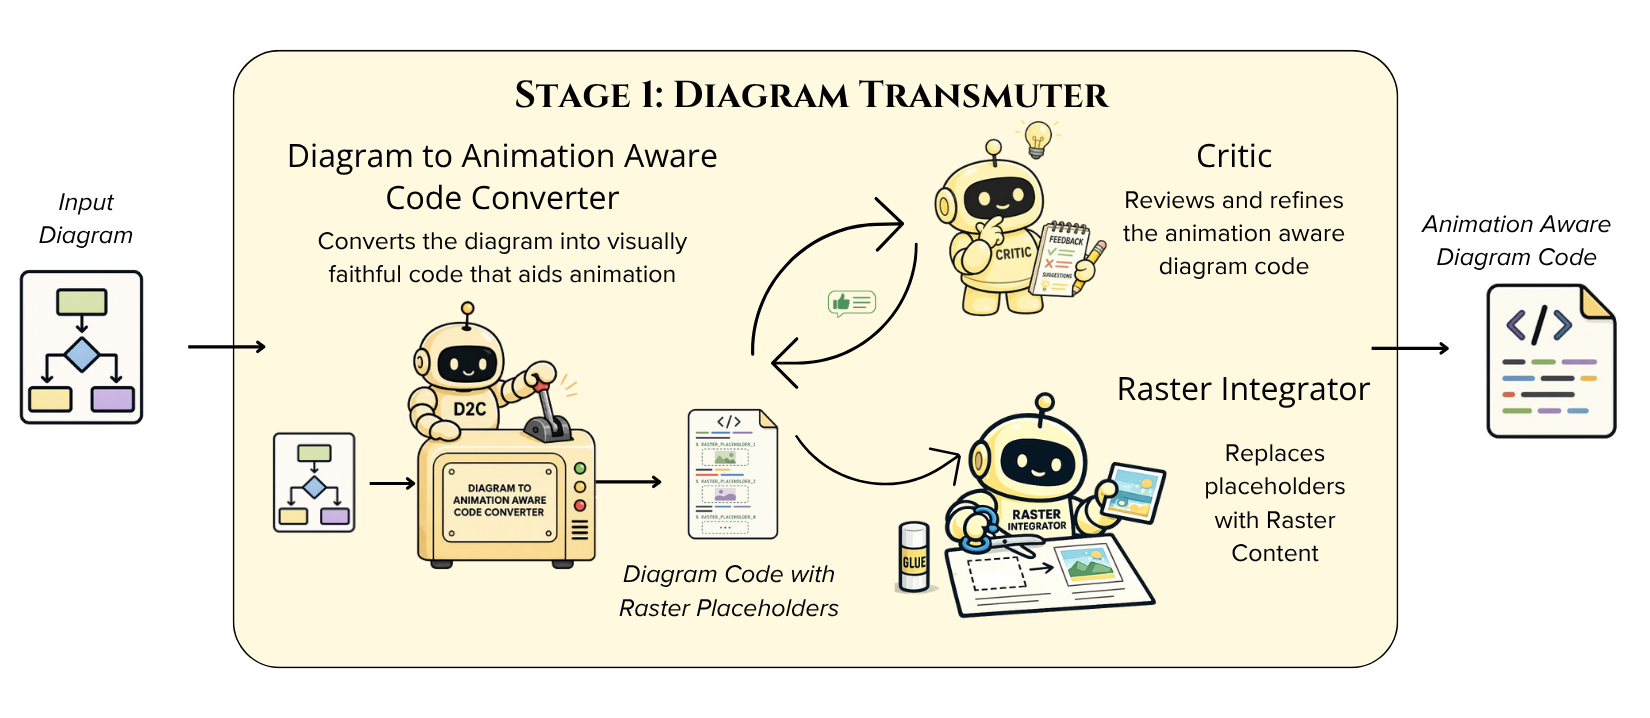
\includegraphics[width=\linewidth]{pipeline_diagrams/Diagram Transmuter.png}
% % %     % \vspace{-0.35cm}
% % %     \caption{An Illustrative Overview of our Diagram Animator Module}
% % %     \vspace{-0.35cm}
% % %     \label{fig:transmuter}
% % % \end{figure}

% % % \subsection{Footnotes}

% % % Indicate footnotes with a number\footnote{Sample of the first footnote} in the
% % % text. Place the footnotes at the bottom of the page on which they appear.
% % % Precede the footnote with a horizontal rule of 2~inches
% % % (12~picas).\footnote{Sample of the second footnote}

% % % \subsection{Figures}

% % % All artwork must be neat, clean, and legible. Lines should be dark
% % % enough for purposes of reproduction; art work should not be
% % % hand-drawn. The figure number and caption always appear after the
% % % figure. Place one line space before the figure caption, and one line
% % % space after the figure. The figure caption is lower case (except for
% % % first word and proper nouns); figures are numbered consecutively.

% % % Make sure the figure caption does not get separated from the figure.
% % % Leave sufficient space to avoid splitting the figure and figure caption.

% % % You may use color figures.
% % % However, it is best for the
% % % figure captions and the paper body to make sense if the paper is printed
% % % either in black/white or in color.
% % % \begin{figure}[h]
% % % \begin{center}
% % % %\framebox[4.0in]{$\;$}
% % % \fbox{\rule[-.5cm]{0cm}{4cm} \rule[-.5cm]{4cm}{0cm}}
% % % \end{center}
% % % \caption{Sample figure caption.}
% % % \end{figure}

% % % \subsection{Tables}

% % % All tables must be centered, neat, clean and legible. Do not use hand-drawn
% % % tables. The table number and title always appear before the table. See
% % % Table~\ref{sample-table}.

% % % Place one line space before the table title, one line space after the table
% % % title, and one line space after the table. The table title must be lower case
% % % (except for first word and proper nouns); tables are numbered consecutively.

% % % \begin{table}[t]
% % % \caption{Sample table title}
% % % \label{sample-table}
% % % \begin{center}
% % % \begin{tabular}{ll}
% % % \multicolumn{1}{c}{\bf PART}  &\multicolumn{1}{c}{\bf DESCRIPTION}
% % % \\ \hline \\
% % % Dendrite         &Input terminal \\
% % % Axon             &Output terminal \\
% % % Soma             &Cell body (contains cell nucleus) \\
% % % \end{tabular}
% % % \end{center}
% % % \end{table}

% % % \section{Default Notation}

% % % In an attempt to encourage standardized notation, we have included the
% % % notation file from the textbook, \textit{Deep Learning}
% % % \cite{goodfellow2016deep} available at
% % % \url{https://github.com/goodfeli/dlbook_notation/}.  Use of this style
% % % is not required and can be disabled by commenting out
% % % \texttt{math\_commands.tex}.


% % % \centerline{\bf Numbers and Arrays}
% % % \bgroup
% % % \def\arraystretch{1.5}
% % % \begin{tabular}{p{1in}p{3.25in}}
% % % $\displaystyle a$ & A scalar (integer or real)\\
% % % $\displaystyle \va$ & A vector\\
% % % $\displaystyle \mA$ & A matrix\\
% % % $\displaystyle \tA$ & A tensor\\
% % % $\displaystyle \mI_n$ & Identity matrix with $n$ rows and $n$ columns\\
% % % $\displaystyle \mI$ & Identity matrix with dimensionality implied by context\\
% % % $\displaystyle \ve^{(i)}$ & Standard basis vector $[0,\dots,0,1,0,\dots,0]$ with a 1 at position $i$\\
% % % $\displaystyle \text{diag}(\va)$ & A square, diagonal matrix with diagonal entries given by $\va$\\
% % % $\displaystyle \ra$ & A scalar random variable\\
% % % $\displaystyle \rva$ & A vector-valued random variable\\
% % % $\displaystyle \rmA$ & A matrix-valued random variable\\
% % % \end{tabular}
% % % \egroup
% % % \vspace{0.25cm}

% % % \centerline{\bf Sets and Graphs}
% % % \bgroup
% % % \def\arraystretch{1.5}

% % % \begin{tabular}{p{1.25in}p{3.25in}}
% % % $\displaystyle \sA$ & A set\\
% % % $\displaystyle \R$ & The set of real numbers \\
% % % $\displaystyle \{0, 1\}$ & The set containing 0 and 1 \\
% % % $\displaystyle \{0, 1, \dots, n \}$ & The set of all integers between $0$ and $n$\\
% % % $\displaystyle [a, b]$ & The real interval including $a$ and $b$\\
% % % $\displaystyle (a, b]$ & The real interval excluding $a$ but including $b$\\
% % % $\displaystyle \sA \backslash \sB$ & Set subtraction, i.e., the set containing the elements of $\sA$ that are not in $\sB$\\
% % % $\displaystyle \gG$ & A graph\\
% % % $\displaystyle \parents_\gG(\ervx_i)$ & The parents of $\ervx_i$ in $\gG$
% % % \end{tabular}
% % % \vspace{0.25cm}


% % % \centerline{\bf Indexing}
% % % \bgroup
% % % \def\arraystretch{1.5}

% % % \begin{tabular}{p{1.25in}p{3.25in}}
% % % $\displaystyle \eva_i$ & Element $i$ of vector $\va$, with indexing starting at 1 \\
% % % $\displaystyle \eva_{-i}$ & All elements of vector $\va$ except for element $i$ \\
% % % $\displaystyle \emA_{i,j}$ & Element $i, j$ of matrix $\mA$ \\
% % % $\displaystyle \mA_{i, :}$ & Row $i$ of matrix $\mA$ \\
% % % $\displaystyle \mA_{:, i}$ & Column $i$ of matrix $\mA$ \\
% % % $\displaystyle \etA_{i, j, k}$ & Element $(i, j, k)$ of a 3-D tensor $\tA$\\
% % % $\displaystyle \tA_{:, :, i}$ & 2-D slice of a 3-D tensor\\
% % % $\displaystyle \erva_i$ & Element $i$ of the random vector $\rva$ \\
% % % \end{tabular}
% % % \egroup
% % % \vspace{0.25cm}


% % % \centerline{\bf Calculus}
% % % \bgroup
% % % \def\arraystretch{1.5}
% % % \begin{tabular}{p{1.25in}p{3.25in}}
% % % % NOTE: the [2ex] on the next line adds extra height to that row of the table.
% % % % Without that command, the fraction on the first line is too tall and collides
% % % % with the fraction on the second line.
% % % $\displaystyle\frac{d y} {d x}$ & Derivative of $y$ with respect to $x$\\ [2ex]
% % % $\displaystyle \frac{\partial y} {\partial x} $ & Partial derivative of $y$ with respect to $x$ \\
% % % $\displaystyle \nabla_\vx y $ & Gradient of $y$ with respect to $\vx$ \\
% % % $\displaystyle \nabla_\mX y $ & Matrix derivatives of $y$ with respect to $\mX$ \\
% % % $\displaystyle \nabla_\tX y $ & Tensor containing derivatives of $y$ with respect to $\tX$ \\
% % % $\displaystyle \frac{\partial f}{\partial \vx} $ & Jacobian matrix $\mJ \in \R^{m\times n}$ of $f: \R^n \rightarrow \R^m$\\
% % % $\displaystyle \nabla_\vx^2 f(\vx)\text{ or }\mH( f)(\vx)$ & The Hessian matrix of $f$ at input point $\vx$\\
% % % $\displaystyle \int f(\vx) d\vx $ & Definite integral over the entire domain of $\vx$ \\
% % % $\displaystyle \int_\sS f(\vx) d\vx$ & Definite integral with respect to $\vx$ over the set $\sS$ \\
% % % \end{tabular}
% % % \egroup
% % % \vspace{0.25cm}

% % % \centerline{\bf Probability and Information Theory}
% % % \bgroup
% % % \def\arraystretch{1.5}
% % % \begin{tabular}{p{1.25in}p{3.25in}}
% % % $\displaystyle P(\ra)$ & A probability distribution over a discrete variable\\
% % % $\displaystyle p(\ra)$ & A probability distribution over a continuous variable, or over
% % % a variable whose type has not been specified\\
% % % $\displaystyle \ra \sim P$ & Random variable $\ra$ has distribution $P$\\% so thing on left of \sim should always be a random variable, with name beginning with \r
% % % $\displaystyle  \E_{\rx\sim P} [ f(x) ]\text{ or } \E f(x)$ & Expectation of $f(x)$ with respect to $P(\rx)$ \\
% % % $\displaystyle \Var(f(x)) $ &  Variance of $f(x)$ under $P(\rx)$ \\
% % % $\displaystyle \Cov(f(x),g(x)) $ & Covariance of $f(x)$ and $g(x)$ under $P(\rx)$\\
% % % $\displaystyle H(\rx) $ & Shannon entropy of the random variable $\rx$\\
% % % $\displaystyle \KL ( P \Vert Q ) $ & Kullback-Leibler divergence of P and Q \\
% % % $\displaystyle \mathcal{N} ( \vx ; \vmu , \mSigma)$ & Gaussian distribution %
% % % over $\vx$ with mean $\vmu$ and covariance $\mSigma$ \\
% % % \end{tabular}
% % % \egroup
% % % \vspace{0.25cm}

% % % \centerline{\bf Functions}
% % % \bgroup
% % % \def\arraystretch{1.5}
% % % \begin{tabular}{p{1.25in}p{3.25in}}
% % % $\displaystyle f: \sA \rightarrow \sB$ & The function $f$ with domain $\sA$ and range $\sB$\\
% % % $\displaystyle f \circ g $ & Composition of the functions $f$ and $g$ \\
% % %   $\displaystyle f(\vx ; \vtheta) $ & A function of $\vx$ parametrized by $\vtheta$.
% % %   (Sometimes we write $f(\vx)$ and omit the argument $\vtheta$ to lighten notation) \\
% % % $\displaystyle \log x$ & Natural logarithm of $x$ \\
% % % $\displaystyle \sigma(x)$ & Logistic sigmoid, $\displaystyle \frac{1} {1 + \exp(-x)}$ \\
% % % $\displaystyle \zeta(x)$ & Softplus, $\log(1 + \exp(x))$ \\
% % % $\displaystyle || \vx ||_p $ & $\normlp$ norm of $\vx$ \\
% % % $\displaystyle || \vx || $ & $\normltwo$ norm of $\vx$ \\
% % % $\displaystyle x^+$ & Positive part of $x$, i.e., $\max(0,x)$\\
% % % $\displaystyle \1_\mathrm{condition}$ & is 1 if the condition is true, 0 otherwise\\
% % % \end{tabular}
% % % \egroup
% % % \vspace{0.25cm}


% % % %A number of width problems arise when LaTeX cannot properly hyphenate a
% % % line. Please give LaTeX hyphenation hints using the \verb+\-+ command.

% % \begin{table*}[t]
% % \centering
% % \caption{\textbf{Evaluation on AnimateBench.}
% % RS: Render Success; VF: Visual Fidelity; CC: Content Coverage;
% % SC: Style Compliance; EF1: Element F1; SS: Selection Sensibility;
% % PG: Presentation Granularity; TC: Traversal Compliance;
% % EntF1: Entity F1; PA: Parent Assignment Accuracy; EdgeF1: Edge Topology F1.
% % Higher is better. Best results are in bold.}
% % \label{tab:main_results}
% % \small
% % \setlength{\tabcolsep}{5pt}

% % \resizebox{\textwidth}{!}{%
% % \begin{tabular}{lccccccccccc}
% % \toprule
% % &
% % \multicolumn{4}{c}{\textbf{Final Narrative}} &
% % \multicolumn{4}{c}{\textbf{Animation Sequence}} &
% % \multicolumn{3}{c}{\textbf{Structure}} \\
% % \cmidrule(lr){2-5}
% % \cmidrule(lr){6-9}
% % \cmidrule(lr){10-12}

% % \textbf{Method}
% % & \texttt{RS}
% % & \texttt{VF}
% % & \texttt{CC}
% % & \texttt{SC}
% % & \texttt{EF1}
% % & \texttt{SS}
% % & \texttt{PG}
% % & \texttt{TC}
% % & \texttt{EntF1}
% % & \texttt{PA}
% % & \texttt{EdgeF1} \\
% % \midrule

% % Baseline A
% % & XX.X & XX.X & XX.X & XX.X
% % & -- & -- & -- & --
% % & -- & -- & -- \\

% % Baseline B
% % & XX.X & XX.X & XX.X & XX.X
% % & XX.X & XX.X & XX.X & XX.X
% % & -- & -- & -- \\

% % \midrule
% % \multicolumn{12}{l}{\textit{Ablations}} \\

% % \textsc{AnimateBanana} w/o Context
% % & XX.X & XX.X & XX.X & XX.X
% % & XX.X & XX.X & XX.X & XX.X
% % & XX.X & XX.X & XX.X \\

% % \textsc{AnimateBanana} w/o Hierarchy
% % & XX.X & XX.X & XX.X & XX.X
% % & XX.X & XX.X & XX.X & XX.X
% % & XX.X & XX.X & XX.X \\

% % \textsc{AnimateBanana} w/o Refinement
% % & XX.X & XX.X & XX.X & XX.X
% % & XX.X & XX.X & XX.X & XX.X
% % & XX.X & XX.X & XX.X \\

% % \midrule
% % \textsc{AnimateBanana}
% % & \textbf{XX.X}
% % & \textbf{XX.X}
% % & \textbf{XX.X}
% % & \textbf{XX.X}
% % & \textbf{XX.X}
% % & \textbf{XX.X}
% % & \textbf{XX.X}
% % & \textbf{XX.X}
% % & \textbf{XX.X}
% % & \textbf{XX.X}
% % & \textbf{XX.X} \\

% % \bottomrule
% % \end{tabular}%
% % }
% % \end{table*}

% \begin{table*}[t]
% \centering
% \definecolor{gateCol}{HTML}{E8F0FE}      % Light Blue for Gates
% \definecolor{gateColDark}{HTML}{C6DAFC}  % Darker Blue for Validity Rate
% \definecolor{qualCol}{HTML}{E6F4EA}      % Light Green for Quality
% \definecolor{qualColDark}{HTML}{CEEAD6}  % Darker Green for Q (Quality Score)
% \definecolor{aansCol}{HTML}{FCE8E6}      % Light Red/Orange for AANS

% \caption{\textbf{Results on AnimateBench (Animated Narrative).}
% Metrics are divided into three colored groups.
% \textbf{Validity Gates (Blue):} VFS: Visual Fidelity Score accuracy \%; ASCS: Animation-Style Compliance Score accuracy \%; Val.\ Rate: Validity Rate.\\
% \textbf{Narrative Quality (Green):} SSS: Selection Sensibility Score; GPS: Granularity and Pacing Score; NAS: Narrative Alignment Score; Q: Aggregate Quality Score.
% \textbf{Final (Red):} AANS: Animated Narrative Score.
% Higher is better for all metrics. Best overall results are in bold.}
% \label{tab:animatebench-narrative-only}
% \small
% \setlength{\tabcolsep}{3.5pt}

% \resizebox{\textwidth}{!}{%
% \begin{tabular}{@{}l c c 
% >{\columncolor{gateCol}}c >{\columncolor{gateCol}}c >{\columncolor{gateColDark}}c 
% >{\columncolor{qualCol}}c >{\columncolor{qualCol}}c >{\columncolor{qualCol}}c >{\columncolor{qualColDark}}c 
% >{\columncolor{aansCol}}c@{}}
% \toprule
% & & &
% \multicolumn{3}{>{\columncolor{gateCol}}c}{\textbf{Validity Gates}} &
% \multicolumn{4}{>{\columncolor{qualCol}}c}{\textbf{Narrative Quality}} &
% \multicolumn{1}{>{\columncolor{aansCol}}c@{}}{\textbf{Final}} \\
% \cmidrule(lr){4-6} \cmidrule(lr){7-10} \cmidrule(l){11-11}

% \textbf{Method} 
% & \textbf{Params} & \textbf{Cost} 
% & \texttt{VFS} acc \% & \texttt{ASCS} acc \% & \textbf{Val.\ Rate} 
% & \texttt{SSS} & \texttt{GPS} & \texttt{NAS} & \textbf{Q} 
% & \textbf{AANS} \\
% \midrule
% \multicolumn{11}{c}{\textbf{Closed-weight models}} \\
% \midrule

% GPT-6-Astra
% & -- & High 
% & XX.X & XX.X & XX.X 
% & XX.X & XX.X & XX.X & XX.X 
% & XX.X \\

% Claude Opus 5 
% & -- & High 
% & XX.X & XX.X & XX.X 
% & XX.X & XX.X & XX.X & XX.X 
% & XX.X \\

% Claude Fable 5 
% & -- & High
% & XX.X & XX.X & XX.X 
% & XX.X & XX.X & XX.X & XX.X 
% & XX.X \\

% Gemini 3.1 Pro 
% & -- & High
% & XX.X & XX.X & XX.X 
% & XX.X & XX.X & XX.X & XX.X 
% & XX.X \\

% \midrule
% \multicolumn{11}{c}{\textbf{Ablation on \textsc{AnimateBanana} backbone}} \\
% \midrule
% \midrule

% Qwen3.8 
% & 27B & Low 
% & XX.X & XX.X & XX.X 
% & XX.X & XX.X & XX.X & XX.X 
% & XX.X \\

% Gemma 4 
% & 31B & Low 
% & XX.X & XX.X & XX.X 
% & XX.X & XX.X & XX.X & XX.X 
% & XX.X \\

% GLM-4.6V 
% & 357B & Low 
% & XX.X & XX.X & XX.X 
% & XX.X & XX.X & XX.X & XX.X 
% & XX.X \\

% Kimi K3 
% & 2.8T & Low 
% & XX.X & XX.X & XX.X 
% & XX.X & XX.X & XX.X & XX.X 
% & XX.X \\

% Qwen3-VL-235B-A22B 
% & 235B & Low
% & XX.X & XX.X & XX.X 
% & XX.X & XX.X & XX.X & XX.X 
% & XX.X \\

% DeepSeek-V4 Pro 
% & 1.6T & Low 
% & XX.X & XX.X & XX.X 
% & XX.X & XX.X & XX.X & XX.X 
% & XX.X \\

% \midrule
% \multicolumn{11}{c}{\textbf{\textsc{AnimateBanana} Stage-specific Ablation (\textit{with Gemini 3.7-Flash as the backbone})}} \\
% \midrule
% \midrule

% \multicolumn{11}{l}{\textit{\textbf{Stage 1 Ablation}}} \\
% \midrule

% \textsc{Stage 1} w/o Critic 
% & -- & -- 
% & XX.X & XX.X & XX.X 
% & XX.X & XX.X & XX.X & XX.X 
% & XX.X \\

% \midrule
% \multicolumn{11}{l}{\textit{\textbf{Stage 2 Ablation}}} \\
% \midrule

% \textsc{Stage 2} w/o Diagram Image Input 
% & -- & -- 
% & XX.X & XX.X & XX.X 
% & XX.X & XX.X & XX.X & XX.X 
% & XX.X \\

% \textsc{Sequencer} w/o XML input 
% & -- & -- 
% & XX.X & XX.X & XX.X 
% & XX.X & XX.X & XX.X & XX.X 
% & XX.X \\

% \textsc{Sequencer} w/o Critic 
% & -- & -- 
% & XX.X & XX.X & XX.X 
% & XX.X & XX.X & XX.X & XX.X 
% & XX.X \\

% \textsc{Narration Drafter} w/o Context 
% & -- & -- 
% & XX.X & XX.X & XX.X 
% & XX.X & XX.X & XX.X & XX.X 
% & XX.X \\

% \midrule
% \multicolumn{11}{l}{\textit{\textbf{Stage 3 Ablation}}} \\
% \midrule

% \textsc{Animation Designer} w/o Diagram Image Input 
% & -- & -- 
% & XX.X & XX.X & XX.X 
% & XX.X & XX.X & XX.X & XX.X 
% & XX.X \\

% \textsc{Animation Designer} w/o Critic 
% & -- & -- 
% & XX.X & XX.X & XX.X 
% & XX.X & XX.X & XX.X & XX.X 
% & XX.X \\

% \midrule
% \midrule

% \textsc{AnimateBanana} 
% & -- & -- 
% & \textbf{XX.X} & \textbf{XX.X} & \textbf{XX.X} 
% & \textbf{XX.X} & \textbf{XX.X} & \textbf{XX.X} & \textbf{XX.X} 
% & \textbf{XX.X} \\

% \midrule

% \textsc{Original Presentations} 
% & -- & -- 
% & \textbf{XX.X} & \textbf{XX.X} & \textbf{XX.X} 
% & \textbf{XX.X} & \textbf{XX.X} & \textbf{XX.X} & \textbf{XX.X} 
% & \textbf{XX.X} \\

% \bottomrule
% \end{tabular}%
% }
% \end{table*}



\section{Evaluation Metrics}
\label{sec:metrics}

\begin{figure*}[t]
    \centering
    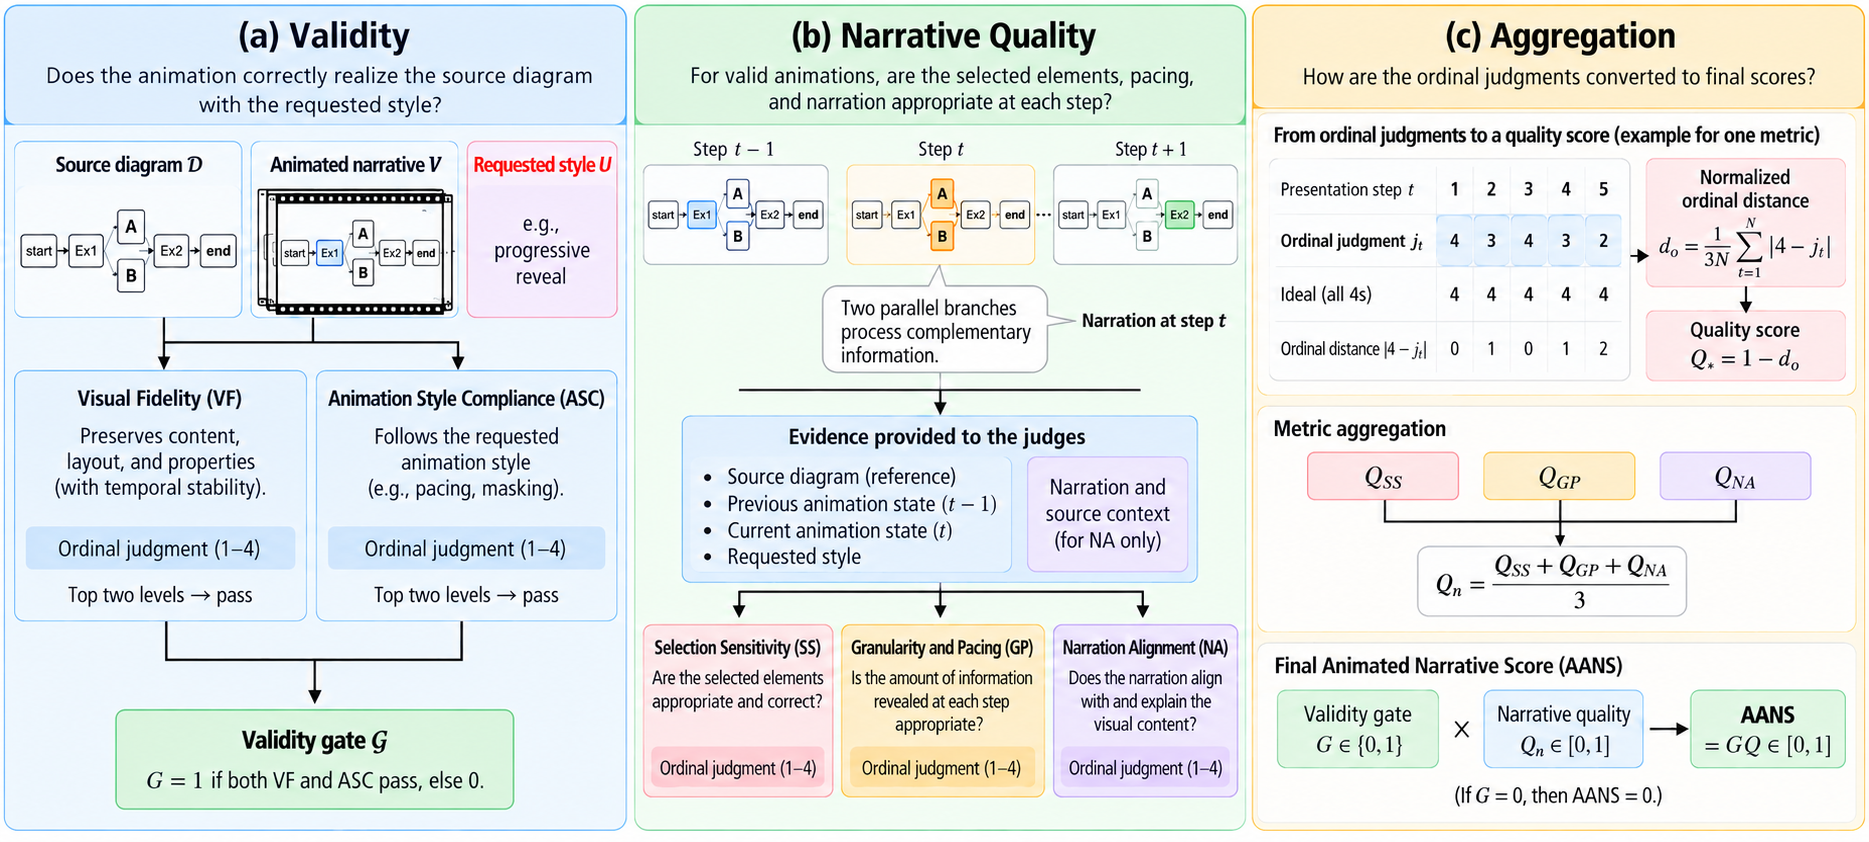
\includegraphics[width=\textwidth]{pipeline_diagrams/AnimateBench-metrics_new.png}
    \caption{\textbf{Evaluation protocol for animated narratives.}
    \textbf{(a) Validity:} Visual Fidelity (VF) measures whether the animated output preserves the source diagram, while Animation Style Compliance (ASC) measures adherence to the requested animation style. Both are evaluated using ordinal judgments and converted to binary pass/fail decisions; the validity gate $G$ passes only when both criteria pass.
    \textbf{(b) Narrative Quality:} For valid animations, each presentation step is evaluated for Selection Sensibility (SS), Granularity and Pacing (GP), and Narration Alignment (NA) using the diagram structure, evolving animation state, and, for NA, narration and source context.
    \textbf{(c) Aggregation:} Step-level ordinal judgments are converted to normalized quality scores $Q_{\mathrm{SS}}$, $Q_{\mathrm{GP}}$, and $Q_{\mathrm{NA}}$, whose average gives narrative quality $Q$. The final Animated Narrative Score is $\mathrm{AANS}=GQ$.}
    \label{fig:eval_metrics}
\end{figure*}

Evaluating an animated scientific diagram requires separating basic validity
from presentation quality. An animation that substantially alters the source
diagram or violates the requested animation style should not receive a high
score merely because its presentation sequence appears coherent. We therefore
use a two-stage evaluation: generated animations must first satisfy
\emph{visual fidelity} and \emph{animation-style compliance} gates, after
which we assess the quality of their visual progression and narration.
Figure~\ref{fig:eval_metrics} summarizes the evaluation protocol.

\noindent \textbf{Validity:}
We use two video-level validity criteria. \textbf{Visual Fidelity (VF)}
evaluates whether the animated output preserves source diagram's content,
layout, geometry, proportions, typography, and visual appearance while
remaining temporally stable. \textbf{Animation Style Compliance (ASC)}
evaluates whether requested animation style is applied consistently
according to its defining behavior. Each criterion receives a four-level
ordinal judgment, with the upper two levels constituting a pass and the lower
two a failure. For an animation $Y$, we define
$G(Y)
=
\mathbbm{1}[\mathrm{VF}(Y)\text{ passes}]
\,
\mathbbm{1}[\mathrm{ASC}(Y)\text{ passes}],
$ such that $G(Y)=1$ only when both validity requirements are satisfied.

\noindent \textbf{Narrative quality:}
For valid animations, we evaluate each presentation step along three
complementary dimensions. \textbf{Selection Sensibility (SS)} assesses
whether elements selected at current step form an appropriate and
structurally coherent focus. \textbf{Granularity and Pacing (GP)} assesses
whether the amount and intrinsic complexity of information introduced
together form an appropriate presentation unit. \textbf{Narration
Alignment (NA)} assesses whether the accompanying narration is temporally
aligned with the active visual content and provides a coherent, contextually
grounded explanation. Each metric is judged at every presentation step using
a four-level ordinal scale.

\noindent \textbf{Aggregation:}
Let $r_t^m \in \{1,2,3,4\}$ denote the ordinal judgment for metric
$m\in\{\mathrm{SS},\mathrm{GP},\mathrm{NA}\}$ at presentation step $t$,
where $4$ denotes the highest-quality judgment. For an animation containing
$N$ evaluated steps, we measure its normalized ordinal distance from the
ideal sequence as 
$d_m
=
\frac{1}{3N}
\sum_{t=1}^{N}
\left|4-r_t^m\right|,
$ and define the corresponding quality score as 
$Q_m = 1-d_m$. 

The overall narrative-quality score is
$
Q
=
\frac{
Q_{\mathrm{SS}}+
Q_{\mathrm{GP}}+
Q_{\mathrm{NA}}
}{3},
$ and the final \textbf{Animated Narrative Score (AANS)} is
$\mathrm{AANS}(Y)=G(Y)\,Q(Y)$ with $\mathrm{AANS}\in[0,1]
$. We report the VF and ASC pass rates, overall validity rate, the three
narrative-quality components, their aggregate $Q$, and AANS. Detailed judging
rubrics, model configurations, animation-style adapters, and aggregation
examples are provided in the supplementary material.

\begin{table*}[t]
\centering

\definecolor{gateCol}{HTML}{E8F0FE}      % Light blue: validity
\definecolor{gateColDark}{HTML}{C6DAFC}  % Darker blue: joint validity
\definecolor{qualCol}{HTML}{E6F4EA}      % Light green: narrative quality
\definecolor{qualColDark}{HTML}{CEEAD6}  % Darker green: aggregate Q
\definecolor{aansCol}{HTML}{FCE8E6}      % Light red/orange: AANS

\caption{\textbf{Results on \textsc{AnimateBench} for animated-narrative generation.}
\textbf{Validity (blue):} VF and ASC denote the fractions of outputs passing
Visual Fidelity and Animation Style Compliance, respectively; Valid.\ denotes
the fraction passing both validity checks.
\textbf{Narrative Quality (green):} SS, GP, and NA denote Selection
Sensibility, Granularity and Pacing, and Narration Alignment, respectively;
these metrics and their aggregate $Q$ are computed over valid outputs.
\textbf{Overall (red):} AANS is the validity-gated Animated Narrative Score,
$\mathrm{AANS}=GQ$, averaged over all outputs, with invalid outputs contributing
zero. All metrics lie in $[0,1]$; higher is better. Best overall results are
shown in bold.}
\label{tab:animatebench-narrative-only}

\small
\setlength{\tabcolsep}{3.5pt}

\resizebox{\textwidth}{!}{%
\begin{tabular}{@{}l c
>{\columncolor{gateCol}}c
>{\columncolor{gateCol}}c
>{\columncolor{gateColDark}}c
>{\columncolor{qualCol}}c
>{\columncolor{qualCol}}c
>{\columncolor{qualCol}}c
>{\columncolor{qualColDark}}c
>{\columncolor{aansCol}}c@{}}

\toprule

& &
\multicolumn{3}{>{\columncolor{gateCol}}c}{\textbf{Validity}} &
\multicolumn{4}{>{\columncolor{qualCol}}c}{\textbf{Narrative Quality}} &
\multicolumn{1}{>{\columncolor{aansCol}}c@{}}{\textbf{Overall}} \\

\cmidrule(lr){3-5}
\cmidrule(lr){6-9}
\cmidrule(l){10-10}

\textbf{Method}
& \textbf{Params}
& \textbf{VF}$\uparrow$
& \textbf{ASC}$\uparrow$
& \textbf{Valid.}$\uparrow$
& \textbf{SS}$\uparrow$
& \textbf{GP}$\uparrow$
& \textbf{NA}$\uparrow$
& $\mathbf{Q}\uparrow$
& \textbf{AANS}$\uparrow$ \\

\midrule
\multicolumn{10}{c}{\textbf{Closed-weight models}} \\
\midrule

GPT-6-Astra
& --
& XX.XXX & XX.XXX & XX.XXX
& XX.XXX & XX.XXX & XX.XXX & XX.XXX
& XX.XXX \\

Claude Opus 5
& --
& XX.XXX & XX.XXX & XX.XXX
& XX.XXX & XX.XXX & XX.XXX & XX.XXX
& XX.XXX \\

Claude Fable 5
& --
& XX.XXX & XX.XXX & XX.XXX
& XX.XXX & XX.XXX & XX.XXX & XX.XXX
& XX.XXX \\

Gemini 3.1 Pro
& --
& XX.XXX & XX.XXX & XX.XXX
& XX.XXX & XX.XXX & XX.XXX & XX.XXX
& XX.XXX \\

\midrule
\multicolumn{10}{c}{
\textbf{Ablation on \textsc{AnimateBanana} backbone}
} \\
\midrule

Qwen3.8
& 27B
& 0.8131 & 0.6703 & 0.5604
& 0.44091 & 0.5162 & 0.4312 & 0.4614
& 0.4614 \\

Gemma 4
& 31B
& 0.3738 & 0.4302 & 0.2441
& 0.1759 & 0.2355 & 0.196184 & 0.2025
& 0.2025 \\

GLM-4.6V
& 357B
& 0.0229 & 0.1609 & 0.0229
& 0.0205 & 0.0234 & 0.0138 & 0.01286
& 0.0128 \\

Kimi K3
& 2.8T
& XX.XXX & XX.XXX & XX.XXX
& XX.XXX & XX.XXX & XX.XXX & XX.XXX
& XX.XXX \\

Qwen3-VL-235B-A22B
& 235B
& 0.0219 & 0.1648 & 0.0109
& 0.0088 & 0.0122 & 0.0088 & 0.01
& 0.01 \\

DeepSeek-V4 Pro
& 1.6T
& XX.XXX & XX.XXX & XX.XXX
& XX.XXX & XX.XXX & XX.XXX & XX.XXX
& XX.XXX \\

\midrule
\multicolumn{10}{c}{
\textbf{\textsc{AnimateBanana} Stage-specific Ablations
(\textit{Gemini 3.7-Flash backbone})}
} \\
\midrule

\multicolumn{10}{l}{\textit{\textbf{Stage 1 Ablation}}} \\
\midrule

\textsc{Stage 1} w/o Critic
& --
& 0.9560 & 0.8571 & 0.8571
& 0.7784 & 0.8161 & 0.8071 & 0.8006
& 0.8006 \\

\midrule
\multicolumn{10}{l}{\textit{\textbf{Stage 2 Ablations}}} \\
\midrule

\textsc{Stage 2} w/o Diagram Image Input
& --
& 0.9450 & 0.8461 & 0.8461
& 0.7679 & 0.8070 & 0.7831 & 0.7860
& 0.7860\\

\textsc{Sequencer} w/o XML Input
& --
& 0.9230 & 0.8241 & 0.8241
& 0.7440 & 0.7803 & 0.7596 &  0.7613 & 0.7613 \\

\textsc{Sequencer} w/o Critic
& --
& 0.9667 & 0.9111 & 0.9111
& 0.8247 & 0.8670 & 0.8534 & 0.8484
& 0.8484 \\

\textsc{Narration Drafter} w/o Context
& --
& 0.9670 & 0.9011 & 0.9011
& 0.8128 & 0.8318 & 0.8222 & 0.8223
& 0.8223 \\

\midrule
\multicolumn{10}{l}{\textit{\textbf{Stage 3 Ablations}}} \\
\midrule

\textsc{Animation Designer} w/o Diagram Image Input
& --
& 0.9560 & 0.8791 & 0.8791
& 0.7938 & 0.8370 & 0.8302 & 0.8203
& 0.8203 \\

\textsc{Animation Designer} w/o Critic
& --
& XX.XXX & XX.XXX & XX.XXX
& XX.XXX & XX.XXX & XX.XXX & XX.XXX
& XX.XXX \\

\midrule

\textsc{AnimateBanana} (without any critics)
& --
& 0.9560
& 0.9011
& 0.8681
& 0.7864
& 0.8258
& 0.8174
& 0.8087
& 0.8087 \\

\midrule
\textsc{AnimateBanana} 
& --
& \textbf{0.9670}
& \textbf{0.9340}
& \textbf{0.9340}
& \textbf{0.8476}
& \textbf{0.8901}
& \textbf{0.8797}
& \textbf{0.8725}
& \textbf{0.8725} \\

\midrule

\textsc{Original Presentations}
& --
& XX.XXX & XX.XXX & XX.XXX
& XX.XXX & XX.XXX & XX.XXX & XX.XXX
& XX.XXX \\

\bottomrule
\end{tabular}%
}
\end{table*}

\section{Experiments}
\label{sec:experiments}

\paragraph{Experimental setup.}
We evaluate \textsc{AnimateBanana} on AnimateBench through automatic
evaluation, ablations, and a user study. Baselines are evaluated either
\emph{end-to-end}, using their final generated animation, or
\emph{pipeline-integrated}, by replacing the corresponding
\textsc{AnimateBanana} components. All methods are therefore comparable on
final-animation metrics, while intermediate metrics are reported only when
the corresponding artifacts are available. We compare against 17 baselines, using Gemini-3.5-Flash as the foundational backbone for \textsc{AnimateBanana} in all applicable pipeline stages.  Unless otherwise stated, methods
receive the same source diagram and available auxiliary context. VLM-based
metrics use \texttt{Qwen3-235B-A22B} with fixed evaluation rubrics. Model configurations,
prompts, baseline adaptations, judge rubrics, and execution details are
provided in the supplementary material.

\paragraph{Evaluation protocol.}
We report the metrics from Sec.~\ref{sec:metrics} on full \textsc{AnimateBench} The main evaluation compares final animated
narratives across methods and, where available, evaluates their intermediate
representations. We additionally ablate \textit{Context} and \textit{Critic-Mediated Feedback} to isolate key design choices. Finally, our user study
complements the automatic metrics with human judgments of animation and
narrative quality, system preference, the utility of auxiliary context, and
the effect of human verification in AnimateBench. The complete study protocol
and additional analyses are provided in the supplementary material.



\subsection{Results}
\label{sec:results}

\paragraph{Final animation quality.}
Table~\ref{tab:main_results} summarizes the evaluation on AnimateBench.
At the final-narrative level, \textsc{AnimateBanana} improves over the strongest baseline by XX.X and
XX.X points on \texttt{Content Coverage} and \texttt{Style Compliance},
respectively. Its \texttt{Visual Fidelity} of XX.X further indicates that
progressively transforming and animating the diagram does not substantially
compromise its source appearance. Together, these results show that the system
retains diagram content while realizing the requested animation behavior.

\paragraph{Presentation planning and structure.}
The intermediate results help explain the final-animation performance.
\textsc{AnimateBanana} achieves XX.X \texttt{Selection Sensibility} and XX.X
\texttt{Traversal Compliance}, indicating that the Animation Planner forms
coherent presentation units and follows the requested style-specific traversal.
Upstream, XX.X \texttt{Entity F1}, XX.X \texttt{Parent Assignment Accuracy},
and XX.X \texttt{Edge Topology F1} show that the structured representation
preserves the entities, hierarchy, and connectivity required for this
planning. These results support the explicit decomposition from structured
diagram representation to presentation planning and style-conditioned
animation.

\paragraph{Effect of design choices.}
The ablations in Table~\ref{tab:main_results} further isolate the contributions
of the major design choices. Removing hierarchy primarily reduces
\texttt{Selection Sensibility} and \texttt{Traversal Compliance}
(XX.X$\rightarrow$XX.X and XX.X$\rightarrow$XX.X), supporting the use of
hierarchical structure for presentation planning. Removing refinement produces
the largest degradation in \texttt{Visual Fidelity} and \texttt{Content
Coverage} (XX.X$\rightarrow$XX.X and XX.X$\rightarrow$XX.X), demonstrating
the importance of iterative correction before animation. Removing source
context has a smaller aggregate effect (XX.X$\rightarrow$XX.X on
\texttt{Selection Sensibility}), with its benefit concentrated on diagrams
whose interpretation depends on information beyond the figure itself; we
analyze this effect separately in the user study. Detailed style-wise,
code-level, and diagnostic results are provided in the supplementary material.

% ============================================================
% USER STUDY
% ============================================================

\subsection{User Study}
\label{subsec:user_study}

We complement the automatic evaluation with a user study involving $n=XX$
participants and XX source diagrams. Participants evaluated animated
narratives with the source diagram available throughout the trial. We measure
absolute perceived quality and three blinded pairwise comparisons:
\textsc{AnimateBanana} against the alternate baseline, generation with versus
without auxiliary context, and human-verified versus pre-verification
AnimateBench narratives. Participants additionally reported their familiarity
with each diagram's topic. Full recruitment, stimulus-selection, assignment,
quality-control, and questionnaire details are provided in the supplementary
material.


\begin{table}[t]
\centering
\caption{\textbf{Absolute human evaluation of \textsc{AnimateBanana}.}
Ratings use a 5-point scale and are reported as mean with 95\% confidence
intervals.}
\label{tab:user_absolute}
\small
\setlength{\tabcolsep}{7pt}
\begin{tabular}{lc}
\toprule
\textbf{Dimension} & \textbf{Rating} \\
\midrule
Content coverage    & X.XX $\pm$ X.XX \\
Animation quality   & X.XX $\pm$ X.XX \\
Style adherence     & X.XX $\pm$ X.XX \\
Presentation flow   & X.XX $\pm$ X.XX \\
Narration alignment & X.XX $\pm$ X.XX \\
Overall quality     & X.XX $\pm$ X.XX \\
\bottomrule
\end{tabular}
\end{table}


\begin{figure}[t]
    \centering
    \includegraphics[width=\linewidth]{figures/userstudy_pairwise.pdf}
    \caption{\textbf{Pairwise human evaluation.}
    Preference distributions for system comparison
    (\textsc{AnimateBanana} vs.\ baseline), context ablation
    ($+K$ vs.\ $-K$), and AnimateBench verification
    (verified vs.\ pre-verification). ``No pref.'' denotes no preference.}
    \label{fig:userstudy_pairwise}
\end{figure}


\paragraph{Perceived narrative quality.}
As shown in Table~\ref{tab:user_absolute}, participants rate
\textsc{AnimateBanana} positively across both visual and narrative dimensions,
with an overall-quality rating of X.XX/5. In particular, ratings of X.XX for
\emph{presentation flow} and X.XX for \emph{narration alignment} indicate that
the generated presentation sequence and accompanying narration are perceived
as coherent with the visual progression. The X.XX rating for
\emph{style adherence} further agrees with the automatic style-compliance
evaluation.

\paragraph{Pairwise comparisons.}
Figure~\ref{fig:userstudy_pairwise} summarizes the blinded comparisons.
Participants prefer \textsc{AnimateBanana} to the alternate baseline in XX.X\%
of trials, compared with XX.X\% for the baseline and XX.X\% with no
preference. This provides human evidence that the improvements observed in the
automatic evaluation translate to perceived differences in the resulting
animated narratives.

Auxiliary context is preferred in XX.X\% of context-ablation trials overall,
with the preference increasing to XX.X\% for context-dependent diagrams.
This supports using caption and paper context selectively: its benefit is
largest when information required for an effective narrative is not explicit
in the diagram itself. Detailed results by context dependence are provided in
the supplementary material.

Finally, human-verified AnimateBench narratives are preferred to their
pre-verification counterparts in XX.X\% of trials, versus XX.X\% for the
unverified versions. The preference is strongest for examples requiring
[SEQUENCE/NARRATION/ANIMATION/MULTIPLE] corrections. This provides direct
evidence that the human-verification stage improves the perceived quality of
the benchmark narratives rather than merely modifying their intermediate
annotations.

\section{Conclusion}

We introduce \emph{animated narrative generation for scientific process diagrams} as a new
task. \textsc{AnimateBanana} provides a
first systematic approach to this task through symbolic, animation-aware
diagram representations, explicit intermediate representations for structure
and presentation, and multimodal agents with critics that progressively
construct and refine the animated narrative. \textbf{AnimateBench} is a
large-scale benchmark for the task, retaining both final narratives and their
intermediate artifacts, while our metrics enable evaluation at multiple levels
of the generation process.
Beyond establishing the task, \textsc{AnimateBanana} reduces the manual effort
of creating animated scientific explanations while retaining control over
content, presentation, narration, and animation style. These capabilities
can complement paper-to-content systems, bringing animated narratives into
automatically generated talks, slides, tutorials, and other explanatory media. More broadly, AnimateBanana opens a creative and sustainable path towards creation of grounded content that is easier to explain, more engaging to consume, and more effective for science communication.


%We expect this work to help move scientific figures from static illustrations
%toward structured, adaptable narratives that can explain themselves.

\section*{Reproducibility statement}

It is important that the work published in ICLR is reproducible. Authors are strongly encouraged to include a paragraph-long Reproducibility Statement at the end of the main text (before references) to discuss the efforts that have been made to ensure reproducibility. This paragraph should not itself describe details needed for reproducing the results, but rather reference the parts of the main paper, appendix, and supplemental materials that will help with reproducibility. For example, for novel models or algorithms, a link to an anonymous downloadable source code can be submitted as supplementary materials; for theoretical results, clear explanations of any assumptions and a complete proof of the claims can be included in the appendix; for any datasets used in the experiments, a complete description of the data processing steps can be provided in the supplementary materials. Each of the above are examples of things that can be referenced in the reproducibility statement. This optional reproducibility statement is not part of the main text and therefore will not count toward the page limit. 

\section*{Ethics statement}

 If authors feel that their paper submission raises questions regarding the Code of Ethics, they are encouraged to include a paragraph of Ethics Statement (at the end of the main text before references) to address potential concerns where appropriate. Topics include, but are not limited to, studies that involve human subjects, practices to data set releases, potentially harmful insights, methodologies and applications, potential conflicts of interest and sponsorship, discrimination/bias/fairness concerns, privacy and security issues, legal compliance, and research integrity issues (e.g., IRB, documentation, research ethics). The optional ethics statement will not count toward the page limit, but should not be more than 1 page.

We acknowledge the significant ethical considerations associated with powerful generative technologies like \textsc{AutoFigure}. The primary risk involves the potential for misuse, where the system could be used to generate scientifically plausible but factually incorrect or misleading schematics to support false claims. To mitigate this risk, we are committed to a policy of transparency and responsible deployment. Our mitigation strategy is twofold. First, we explicitly declare that \textsc{AutoFigure} is an assistive tool with limitations. This disclaimer, stating that the system is not a substitute for expert verification and may not produce perfectly reliable outputs, will be placed prominently within this paper and in the README file of the public code repository. Second, the open-source license governing \textsc{AutoFigure} will include a mandatory attribution clause. This clause requires any academic publication using a figure generated by our tool to (a) include a specific section that discusses the role AI played in the work, and (b) explicitly caption the figure as having been generated by \textsc{AutoFigure}. These requirements are designed to ensure transparency and accountability in the downstream use of our technology, fostering a research environment where AI tools are used to augment, not compromise, scientific integrity.

\section{AI Use Statement}

we require authors to disclose AI use in a mandatory section in their paper (this section will not be counted towards the page limit). The ICLR paper template includes a boilerplate disclosure to give authors a sense of the expected detail. You are not required to follow this format exactly—we believe these disclosures may be a source of useful information to the community about how AI is affecting research workflows, and we encourage you to provide as much detail as you want!

Ultimately the paper’s authors are responsible for the contents of their submissions. Consequently, a substantial falsehood, instance of plagiarism, or misrepresentation produced by an LLM would be considered a Code of Ethics violation on the part of the paper’s authors, and might lead to desk rejection of the paper. 

Example AI disclosure section
In this work, we used generative AI tools for <tasks with required disclosure>. We have not used generative AI tools for <other tasks with required disclosure>, and <the rest of the required disclosure tasks> are not applicable to this work. Additionally, we used generative AI tools for <tasks with recommended disclosure>. We have reviewed all AI-assisted work. [Elaborate. For example, “we checked LLM-generated research ideas for potential plagiarism through a manual literature survey”, “LLM-generated code was verified and tested for correctness by 2 authors”, etc.]. We take responsibility for the final content of this work, including text, claims or artifacts produced with the aid of generative AI.

Below, we share a list of common research subtasks along with the necessity of disclosing them in the paper manuscript.

Required: Generate synthetic data sets, help develop theoretical models or conceptual frameworks, formulate mathematical claims, provide critical ingredients for proving mathematical claims, assist in the writing of proofs, propose or refine hypotheses, design or provide feedback on research  methodology or experiments, implement methods, assist with translation, clean and reformat dataset, support qualitative and thematic data analysis, interpret results. 

Recommended: Formulate questions for surveys or interviews, create or modify scientific figures or images, suggest experimental parameters, create or edit software code,  creation of artifacts, draft parts of a research paper, transcribe recordings of research material, summarize or analyse existing literature, discover research topics or identify gaps, brainstorming, sourcing/searching for information, edit a research paper to improve readability, identify relevant literature, format references, suggest a structure for a research paper, propose a title or keywords for a research paper.

LLMs were utilized as assistive tools at various stages of this research and manuscript preparation to enhance productivity and quality. Our use of these tools was supervised, with the final responsibility for all content resting with the human authors. In the initial phase of our work, we employed LLM-based tools to assist with literature discovery. These tools helped in identifying and summarizing a broad range of relevant prior work, which facilitated a comprehensive understanding of the existing research landscape. During the implementation of the \textsc{AutoFigure} framework, we utilized Claude to assist in writing and refining code segments. This process accelerated development and helped in debugging and optimizing our software components. For the preparation of the manuscript, LLMs (e.g. Gemini-2.5-Pro) were used for text polishing, including improving grammatical correctness, clarity, and readability. The core scientific ideas, methodologies, and arguments presented in this paper were conceived and articulated by the authors. Finally, upon completion of the draft, we subjected the manuscript to a secondary review process using the DeepReviewer \citep{zhu2025deepreview} model. This tool helped to proactively identify potential weaknesses in our argumentation, experimental setup, and presentation. We carefully considered the feedback provided by DeepReviewer and made targeted revisions to address the concerns we deemed valid, thereby strengthening the final version of this paper.


\bibliography{iclr2027_conference}
\bibliographystyle{iclr2027_conference}


\section{Appendix}

\subsection{Implementation Details for AnimateBanana}

\textsc{AnimateBanana} supports SVG, as the underlying representation for diagram-to-code conversion and animation. The generated code preserves the mapping with the source diagram's spatial coordinates, assigns semantic identifiers to diagram entities and their relationships, and records semantic and hierarchical metadata. This allows the downstream parser and sequencer to operate over a code-agnostic representation while retaining the language-specific native representation for rendering and animation. The following describes the implementation choices that enable this correspondence.
\subsubsection{Diagram Transmuter: Code-specific Representation}
 In the Diagram Transmuter, the D2C converter first establishes the dimensions of the source image and maps to it component by component in pixel coordinates. This provides a consistent coordinate frame for mapping the generated representation back to the source diagram. The coordinate system is anchored at the top-left of the source image since SVG directly follows the image-space coordinate convention.\\
 For SVG generation, the source image dimensions are directly encoded in the SVG \texttt{viewBox}, providing a one-to-one image-space coordinate frame. Semantic metadata is embedded using HTML5 \texttt{data-*} attributes, with \texttt{data-id}, \texttt{data-class}, and \texttt{data-parent}. Semantic roles are encoded using a fixed vocabulary consisting of blocks, standalone nodes, child nodes, text nodes, raster nodes, composite elements, and edges. Thus, the generated SVG code simultaneously functions as an executable visual programmatic representation and a structured description of the diagram graph.\\ Edges additionally carry \texttt{data-source} and \texttt{data-target} attributes. This explicit metadata is extremely important for SVG since visual elements may have no semantic id that can be reliably referenced during subsequent animation. The DOM is also organized according to rendering order, with background containers preceding edges and foreground nodes and text.\\
 A central design requirement in both representations is that natural images, logos, icons, and other complex raster graphics are represented as explicitly identified \textit{raster nodes}. Rather than asking the diagram-to-code model to attempt to draw these complex raster graphics, the converter inserts a placeholder at the corresponding location and records its identity. The Raster Integrator subsequently extracts the corresponding region from the source diagram and maps it into the placeholder\\
 
 The resulting representation is therefore simultaneously optimized for three requirements: faithful rendering of the source diagram, structural grounding to the original diagram, and semantic grounding for ease of animation and downstream reasoning.
 \subsubsection{Animation Planner: Code-Agnostic Representation}
 The implementation of the Animation Planner begins by transforming the animation-aware SVG representation into the common XML schema. The parser reads the semantic identifiers embedded in the generated code and constructs a language-independent XML representation of the diagram entities, relationships, and hierarchy established during diagram transmutation. The resulting schema records each diagram entity together with its semantic class, identifier, parent, and hierarchy depth. Directed relationships are represented explicitly through source--target references. Composite objects retain their whole-part structure, while raster nodes remain identifiable as independent entities. This representation allows the Sequencer to reason over the diagram at the level of semantic entities rather than individual drawing primitives.\\

 The Sequencer is further constrained by the structural relationships encoded in the schema. Parent-child relationships provide the hierarchy information required to determine whether a module should be introduced as a whole or decomposed into its constituents, while directed edges provide dependencies that constrain permissible traversal orders. The resulting sequence thus represents an ordered traversal over the diagram graph rather than an arbitrary ordering of visual elements. This allows a single animation sequence to be instantiated using different animation styles.

\subsubsection{Diagram Animator: Code-specific Representation}
The animation generator preserves the geometry and semantic identifiers of the original diagram code. It modifies only the visual state of the identified elements according to the animation style and at their scheduled presentation timestamps. Thus, animation does not require repositioning the underlying diagram.\\
The animation is implemented directly over the ID-tagged SVG representation using CSS. The animation generator injects style and keyframe definitions that reference the semantic identifiers produced by the Diagram Transmuter.\\ The narration associated with each sequence step is additionally rendered as a synchronized subtitle layer during animation generation.\\
%The final animation is rendered through the native mechanism of the target representation. For TikZ, the \texttt{animate} package produces an interactive PDF in which the animation frames are embedded directly in the document and can be played using PDF viewers like Adobe Acrobat and Foxit Reader. The generated TikZ can additionally be converted to SVG using \texttt{dvisvgm}, enabling the resulting animation to enter the same browser-based rendering and export pipeline as native SVG animations.

\section{Detailed Evaluation Protocol}
\label{sec:supp_eval}

This section provides the detailed judging protocol underlying the evaluation
metrics introduced in Sec.~\ref{sec:metrics}. We describe the judge
configuration, metric-specific inputs and criteria, ordinal rubrics, and the
aggregation procedure used to obtain the reported scores.

\subsection{Judge Configuration}
\label{sec:supp_eval_setup}

Table~\ref{tab:supp_judge_setup} summarizes the evaluation setup. Visual
Fidelity (VF) and Animation Style Compliance (ASC) operate on the complete
animation, whereas Selection Sensibility (SS), Granularity and Pacing (GP),
and Narration Alignment (NA) are evaluated at individual presentation steps.

\begin{table*}[t]
\centering
\small
\setlength{\tabcolsep}{5pt}
\begin{tabular}{lclp{9.1cm}}
\toprule
\textbf{Metric} & \textbf{Scope} & \textbf{Judge} & \textbf{Inputs} \\
\midrule
VF
& Video
& Gemini 3.6 Flash
& Source diagram, generated animation, and requested animation style. \\

ASC
& Video
& Gemini 3.6 Flash
& Generated animation and requested animation style together with its
style-specific behavioral rules. \\

SS
& Presentation step
& Kimi 2.6
& Source diagram, current rendered state, previous rendered state when
available, ground-truth structural representation, and requested animation
style. \\

GP
& Presentation step
& Kimi 2.6
& Source diagram, current rendered state, previous rendered state when
available, ground-truth structural representation, and requested animation
style. \\

NA
& Presentation step
& Kimi 2.6
& Inputs used for SS/GP together with the step-level narration and available
source-document context. \\
\bottomrule
\end{tabular}
\caption{\textbf{Judge configuration for animated-narrative evaluation.}
VF and ASC assess global animation validity, whereas SS, GP, and NA evaluate
the evolving presentation at individual steps.}
\label{tab:supp_judge_setup}
\end{table*}

For VF, the generated animation is sampled at $2$ FPS. ASC uses $4$ FPS to
better capture short and potentially rapid style-specific transitions. For
SS, GP, and NA, evaluation is performed at presentation steps using the
rendered state corresponding to the current step. Except for the first step,
the preceding rendered state is additionally supplied to the judge.

The requested animation style is provided during evaluation whenever relevant.
This prevents legitimate style-specific transformations from being confused
with generation errors. For example, the bounding box introduced by hopping-
or sliding-box animations should not be interpreted as an extraneous visual
artifact, while grayscale regions in colour-pop animations should not be
interpreted as a failure to preserve source colours.

\subsection{Visual Fidelity}
\label{sec:supp_vf}

Visual Fidelity (VF) assesses whether the generated animation remains faithful
to the source diagram throughout its duration while avoiding temporal
instability or rendering artifacts. The judge considers the following
criteria:

\begin{itemize}
    \item \textbf{Element alteration.}
    Whether diagram elements become distorted, incorrectly morphed, corrupted,
    or otherwise unrecognizable during the animation.

    \item \textbf{Visual-layout fidelity.}
    Whether the overall diagram flow, containment hierarchy, and connections
    remain consistent with the source.

    \item \textbf{Geometric-layout fidelity.}
    Whether spatial arrangement, relative positioning, and alignment remain
    faithful to the source diagram.

    \item \textbf{Proportion and scale fidelity.}
    Whether element dimensions, aspect ratios, and relative scales are
    preserved.

    \item \textbf{Text and typographic integrity.}
    Whether text labels, mathematical notation, and symbols remain accurate
    and legible.

    \item \textbf{Style and appearance.}
    Whether colours and other visual characteristics remain faithful to the
    source, except where modification is explicitly required by the requested
    animation style.
\end{itemize}

VF is assigned a four-level ordinal judgment ranging from high source fidelity
to severe failure. The upper two ordinal levels constitute a validity pass,
whereas the lower two constitute a failure.

\subsection{Animation Style Compliance}
\label{sec:supp_asc}

Animation Style Compliance (ASC) evaluates whether the requested animation
mechanism is applied correctly and consistently throughout the generated
animation. Since different animation styles impose different temporal
behaviours, the judge uses a style-specific checklist.

For the animation styles considered in our experiments, the defining
behaviours are:

\begin{itemize}
    \item \textbf{Progressive Reveal.}
    The animation begins from an empty canvas and progressively accumulates
    diagram elements until the complete diagram is visible. Elements that
    have already been revealed should not subsequently disappear.

    \item \textbf{Alpha Masking.}
    The complete diagram is initially visible in a semi-transparent state,
    with elements progressively emphasized or de-emphasized through opacity
    changes according to the presentation sequence.

    \item \textbf{Colour Pop.}
    The diagram begins in grayscale and selected elements are progressively
    restored to their original colours according to the presentation sequence.

    \item \textbf{Hopping Bounding Box.}
    A bounding box moves discretely between the elements selected by
    successive presentation steps.

    \item \textbf{Sliding Bounding Box.}
    A bounding box moves continuously between the elements selected by
    successive presentation steps.
\end{itemize}

ASC is evaluated using an ordinal rubric representing progressively stronger
compliance with the defining behavior of the requested style. The upper two
levels constitute a pass and correspond to animations that satisfy all
defining rules or exhibit only minor deviations. The lower levels correspond
to substantial or severe violations of the requested style and constitute a
failure. Minor initialization deviations are distinguished from violations of
the core temporal behavior. For example, a progressive-reveal animation that
does not begin from a perfectly blank canvas can still pass when the remaining
animation consistently follows cumulative reveal behavior.

\subsection{Selection Sensibility}
\label{sec:supp_ss}

Selection Sensibility (SS) assesses whether the elements selected at
presentation step $t$ constitute an appropriate logical focus given the
structure of the source diagram. The judgment is conditioned on the current
and previous animation states, the ground-truth structural representation,
and the requested animation style.

SS considers two complementary aspects:

\begin{itemize}
    \item \textbf{Element appropriateness.}
    Whether the newly targeted element or elements are appropriate at the
    current point in the presentation, accounting for the diagram's flow,
    hierarchy, and structural relationships. This criterion also captures
    cases in which a visually valid animation applies the requested animation
    behavior to the wrong elements.

    \item \textbf{Group coherence.}
    When multiple elements are selected together, whether they form a
    meaningful logical group and respect the relevant structural
    dependencies.
\end{itemize}

The four ordinal levels are interpreted as follows:

\begin{enumerate}
    \item[4.] \textbf{Fully sensible.}
    The selected elements form an appropriate and structurally coherent
    presentation focus.

    \item[3.] \textbf{Minor violation.}
    The selection contains small avoidable weaknesses but remains largely
    reasonable.

    \item[2.] \textbf{Major violation.}
    Elements are selected at inappropriate points in the presentation or the
    grouping substantially conflicts with the expected diagram flow.

    \item[1.] \textbf{Severe violation.}
    Element selection is largely arbitrary, groupings are incoherent, or the
    presentation strongly contradicts the diagram hierarchy or flow.
\end{enumerate}

\subsection{Granularity and Pacing}
\label{sec:supp_gp}

Granularity and Pacing (GP) evaluates whether the information introduced at a
presentation step forms an appropriately sized and sufficiently digestible
presentation unit. GP is intentionally separated from SS: SS determines
\emph{which} elements constitute an appropriate focus, whereas GP evaluates
\emph{how much} information is presented together once that focus has been
selected.

The judge considers three factors:

\begin{itemize}
    \item \textbf{Volume.}
    The amount of diagram content introduced together at the current step.
    Sparse presentation is not penalized solely because a step contains few
    elements.

    \item \textbf{Intrinsic complexity.}
    Whether the selected elements are sufficiently complex that presenting
    them simultaneously overloads the step even when the raw number of
    elements is moderate.

    \item \textbf{Explanatory relevance.}
    Whether grouping a comparatively large or complex set of elements is
    justified by the logical or explanatory structure of the diagram.
    Relevance therefore protects structurally meaningful groups from being
    penalized solely because of their size.
\end{itemize}

The four ordinal levels are interpreted as follows:

\begin{enumerate}
    \item[4.] \textbf{Well paced.}
    The amount and intrinsic complexity of the presentation unit are
    appropriate.

    \item[3.] \textbf{Minor overload.}
    The step is somewhat more complex than ideal but remains well justified by
    the presentation flow.

    \item[2.] \textbf{Major overload.}
    A large or intrinsically complex group is introduced together with only
    partial explanatory justification.

    \item[1.] \textbf{Severe overload.}
    The step introduces an unreasonably complex or overloaded presentation
    unit that is not sufficiently justified by the diagram's explanatory
    structure.
\end{enumerate}

\subsection{Narration Alignment}
\label{sec:supp_na}

Narration Alignment (NA) assesses whether the narration associated with
presentation step $t$ appropriately explains the visual content active at that
step. In addition to the inputs used for SS and GP, the judge receives the
step-level narration and available source-document context. The context
contains the paper title, abstract, method section, and figure caption when
available.

NA evaluates three aspects:

\begin{itemize}
    \item \textbf{Transition alignment.}
    Whether the narration addresses the elements currently appearing,
    transitioning, or being emphasized. Narration that discusses previously
    presented material while ignoring the current visual focus is penalized.

    \item \textbf{Narrative and contextual value.}
    Whether the narration provides a useful functional explanation of what the
    active presentation step represents or accomplishes. Merely describing
    visible shapes or labels without explanatory value is insufficient.
    Concise narration is acceptable when it remains informative.

    \item \textbf{Coherence and factuality.}
    Whether the narration is linguistically coherent and consistent with the
    source diagram and provided context, without introducing unsupported
    terminology, incorrect methods, or nonexistent acronyms.
\end{itemize}

The four ordinal levels are interpreted as follows:

\begin{enumerate}
    \item[4.] \textbf{Well aligned and informative.}
    The narration provides a clear, natural, and contextually grounded
    explanation of the active visual content.

    \item[3.] \textbf{Minor flaws.}
    The narration may be somewhat verbose or slightly under-explain the
    current step, but remains aligned and useful.

    \item[2.] \textbf{Major flaws.}
    The narration provides little explanatory value, is predominantly a
    superficial visual description, or suffers from substantial temporal
    misalignment.

    \item[1.] \textbf{Severe flaws.}
    The narration contradicts the active visual content or confidently
    introduces unsupported or hallucinated information.
\end{enumerate}

\subsection{Ordinal Aggregation}
\label{sec:supp_ordinal_aggregation}

For each narrative-quality metric
$m\in\{\mathrm{SS},\mathrm{GP},\mathrm{NA}\}$, let

\[
\mathbf{r}^{m}
=
(r_1^m,\ldots,r_N^m),
\qquad
r_t^m\in\{1,2,3,4\},
\]

denote the sequence of ordinal judgments across the $N$ evaluated
presentation steps, where larger values correspond to higher-quality
judgments. The ideal sequence is

\[
\mathbf{r}^{*}=(4,\ldots,4).
\]

We quantify deviation from this ideal using a normalized ordinal
$\ell_1$ distance:

\[
d_m
=
\frac{1}{3N}
\sum_{t=1}^{N}
\left|r_t^m-r_t^*\right|
=
\frac{1}{3N}
\sum_{t=1}^{N}
\left|4-r_t^m\right|.
\]

The normalization factor $3N$ is the maximum possible distance from the ideal
sequence and therefore gives $d_m\in[0,1]$. The corresponding quality score is

\[
Q_m = 1-d_m.
\]

Consequently, a sequence receiving the highest ordinal judgment at every
presentation step obtains $Q_m=1$, while a sequence receiving the lowest
judgment at every step obtains $Q_m=0$. This aggregation can equivalently be
viewed as a cost-sensitive generalization of Hamming distance: rather than
assigning equal cost to every mismatch with the ideal sequence, each mismatch
is weighted according to its ordinal separation from the highest-quality
judgment.

The aggregate narrative-quality score is obtained by equally weighting the
three component scores:

\[
Q
=
\frac{
Q_{\mathrm{SS}}
+
Q_{\mathrm{GP}}
+
Q_{\mathrm{NA}}
}{3},
\qquad
Q\in[0,1].
\]

\subsection{Validity Gating and Animated Narrative Score}
\label{sec:supp_gating}

Let

\[
g_{\mathrm{VF}}(Y)
=
\mathbb{1}[\mathrm{VF}(Y)\text{ passes}],
\]

and

\[
g_{\mathrm{ASC}}(Y)
=
\mathbb{1}[\mathrm{ASC}(Y)\text{ passes}].
\]

The joint validity indicator is

\[
G(Y)
=
g_{\mathrm{VF}}(Y)
g_{\mathrm{ASC}}(Y).
\]

An animation is therefore considered valid only when it passes both VF and
ASC. The final Animated Narrative Score is

\[
\mathrm{AANS}(Y)
=
G(Y)\,Q(Y),
\qquad
\mathrm{AANS}\in[0,1].
\]

Thus, invalid outputs receive $\mathrm{AANS}=0$ irrespective of their
narrative-quality judgments. This prevents an animation that substantially
violates source fidelity or the requested animation behavior from receiving a
high end-to-end score solely because some aspects of its presentation sequence
appear reasonable.

\subsection{Dataset-Level Reporting}
\label{sec:supp_dataset_reporting}

For a collection of generated animations, we report the following quantities:

\begin{itemize}
    \item \textbf{VF:} the fraction of generated outputs that pass the Visual
    Fidelity criterion;

    \item \textbf{ASC:} the fraction of generated outputs that pass Animation
    Style Compliance;

    \item \textbf{Validity:} the fraction of outputs for which $G=1$, i.e.,
    those passing both VF and ASC;

    \item \textbf{SS, GP, and NA:} the mean corresponding quality scores
    $Q_{\mathrm{SS}}$, $Q_{\mathrm{GP}}$, and $Q_{\mathrm{NA}}$ over valid
    outputs;

    \item \textbf{$Q$:} the mean aggregate narrative-quality score over valid
    outputs; and

    \item \textbf{AANS:} the mean value of $G(Y)Q(Y)$ over all generated
    outputs, with invalid outputs contributing zero.
\end{itemize}

Reporting the validity components separately from narrative quality provides a
more diagnostic view than AANS alone. VF and ASC expose failures in source
preservation and animation-style realization, while SS, GP, and NA distinguish
errors in presentation-unit selection, presentation granularity, and
narration--visual coordination. AANS summarizes these complementary aspects in
a single validity-aware end-to-end score.

\subsection{Judge Prompts and Style Adapters}
\label{sec:supp_judge_prompts}

All VLM judges are instructed to return a single ordinal judgment according to
the metric-specific rubric above. For style-dependent metrics, the prompt is
augmented with a description of the requested animation style and its defining
behavior. This style adapter ensures that identical visual changes can be
interpreted differently when required by the specified animation mechanism.

For SS, GP, and NA, the judge is additionally instructed to reason about the
difference between the previous and current presentation states rather than
assessing the current frame in isolation. For NA, the source-document context
is supplied only as grounding information: narration is expected to remain
aligned with the current visual step and is penalized when contextual
information replaces, contradicts, or distracts from the active presentation
content.

The complete prompts, output schemas, and parsing rules used for all judges
will be released with the evaluation code.


\end{document}

% We will release AnimateBench, evaluation code, prompts and configurations required to reproduce the reported experiments, and a reference implementation of the AnimateBanana pipeline.